%-----------------------------------------
% Note: Use pdflatex to process this file.
%-----------------------------------------

%\documentclass{article}
\documentclass{hitec}

\usepackage{setspace}
\usepackage{graphicx}
\usepackage{moreverb}    % Defines {listing} environment.
\usepackage{amsmath, amsthm, amssymb, amsbsy, mathtools}
\usepackage{alltt}
\usepackage{rotating}
\usepackage{subcaption}
\usepackage{toc-bmad}
\usepackage{xspace}
%%\usepackage{makeidx}
\usepackage[section]{placeins}   % For preventing floats from floating to end of chapter.
\usepackage{longtable}  % For splitting long vertical tables into pieces
\usepackage{index}
\usepackage{multirow}
\usepackage{booktabs}   % For table layouts
\usepackage{yhmath}     % For widehat
\usepackage{xcolor}      % Needed for listings package.
\usepackage{listings}
\usepackage[T1]{fontenc}   % so _, <, and > print correctly in text.
\usepackage[strings]{underscore}    % to use "_" in text
\usepackage[pdftex,colorlinks=true]{hyperref}   % Must be last package!

%----------------------------------------------------------------

\newcommand{\extref}[1]{$\S$\ref*{#1}}   % No hyperlink. For external refs. \extref
\newcommand{\comma}{\> ,}
\newcommand{\period}{\> .}
\newcommand{\wt}{\widetilde}
\newcommand{\grv}{\textasciigrave}
\newcommand{\hyperbf}[1]{\textbf{\hyperpage{#1}}}
\newcommand{\Ss}{\(^*\)}
\newcommand{\Dd}{\(^\dagger\)}

\newcommand{\AND}{&& \hskip -17pt\relax}
\newcommand{\CR}{\\}
\newcommand{\CRNO}{\nonumber \\}
\newcommand{\dstyle}{\displaystyle}

\newcommand{\Begineq}{\begin{equation}}
\newcommand{\Endeq}{\end{equation}}
\newcommand{\NoPrint}[1]{}

\newcommand{\pow}[1]{\cdot 10^{#1}}
\newcommand{\Bf}[1]{{\bf #1}}
\newcommand{\bfr}{\Bf r}

\newcommand{\bmad}{{\sl Bmad}\xspace}
\newcommand{\tao}{{\sl Tao}\xspace}
\newcommand{\mad}{{\sl MAD}\xspace}
\newcommand{\cesr}{{\sl CESR}\xspace}

\newcommand{\sref}[1]{\S\ref{#1}}
\newcommand{\Sref}[1]{Sec.~\sref{#1}}
\newcommand{\cref}[1]{Chapter~\ref{#1}}

\newcommand{\Newline}{\hfil \\ \relax}

\newcommand{\eq}[1]{{(\protect\ref{#1})}}
\newcommand{\Eq}[1]{{Eq.~(\protect\ref{#1})}}
\newcommand{\Eqs}[1]{{Eqs.~(\protect\ref{#1})}}

\newcommand{\vn}{\ttcmd}           % For variable names
\newcommand{\vni}{\ttcmdindx}
\newcommand{\cs}{\ttcmd}           % For code source
\newcommand{\cmd}{\ttcmd}          % For Unix commands
\newcommand{\rn}{\ttcmd}           % For Routine names
\newcommand{\tn}{\ttcmd}           % For Type (structure) names
\newcommand{\bn}[1]{{\bf #1}}       
\newcommand{\toffset}{\vskip 0.01in}
\newcommand{\rot}[1]{\begin{rotate}{-45}#1\end{rotate}}

\newcommand{\data}{{\mbox{data}}}
\newcommand{\reference}{{\mbox{ref}}}
\newcommand{\model}{{\mbox{model}}}
\newcommand{\base}{{\mbox{base}}}
\newcommand{\design}{{\mbox{design}}}
\newcommand{\meas}{{\mbox{meas}}}
\newcommand{\var}{{\mbox{var}}}

\newcommand\ttcmd{\begingroup\catcode`\_=11 \catcode`\%=11 \dottcmd}
\newcommand\dottcmd[1]{\texttt{#1}\endgroup}

\newcommand\ttcmdindx{\begingroup\catcode`\_=11 \catcode`\%=11 \dottcmdindx}
\newcommand\dottcmdindx[1]{\texttt{#1}\endgroup\index{#1}}

\newcommand{\St}{$^{st}$\xspace}
\newcommand{\Nd}{$^{nd}$\xspace}
\newcommand{\Th}{$^{th}$\xspace}
\newcommand{\B}{$\backslash$}
\newcommand{\W}{$^\wedge$}

\newcommand{\cbar}[1]{\overline C_{#1}}

\newlength{\dPar}
\setlength{\dPar}{1.5ex}

\newenvironment{example}
  {\vspace{-3.0ex} \begin{alltt}}
  {\end{alltt} \vspace{-2.5ex}}

\newcommand\Strut{\rule[-2ex]{0mm}{6ex}}

\newenvironment{Itemize}
  {\begin{list}{$\bullet$}
    {\addtolength{\topsep}{-1.5ex} 
     \addtolength{\itemsep}{-1ex}
    }
  }
  {\end{list} \vspace*{1ex}}

\newcommand{\Section}[1]{\section{#1}\indent\vspace{-3ex}}

\newcommand{\SECTION}[1]{\section*{#1}\indent\vspace{-3ex}}

% From pg 64 of The LaTex Companion.

\newenvironment{ventry}[1]
  {\begin{list}{}
    {\renewcommand{\makelabel}[1]{\textsf{##1}\hfil}
     \settowidth{\labelwidth}{\textsf{#1}}
     \addtolength{\itemsep}{-1.5ex}
     \addtolength{\topsep}{-1.0ex} 
     \setlength{\leftmargin}{5em}
    }
  }
  {\end{list}}


\renewcommand{\ttdefault}{txtt}
%\lstset{basicstyle = \small\asciifamily,columns=flexible}  % Enable cut and paste
\lstset{basicstyle = \small} 

\renewcommand{\textfraction}{0.1}
\renewcommand{\topfraction}{1.0}
\renewcommand{\bottomfraction}{1.0}

\settextfraction{0.9}  % Width of text
\setlength{\parindent}{0pt}
\setlength{\parskip}{1ex}
%\setlength{\textwidth}{6in}
\newcommand{\Section}[1]{\section{#1}\vspace*{-1ex}}

\newenvironment{display}
  {\vspace*{-1.5ex} \begin{alltt}}
  {\end{alltt} \vspace*{-1.0ex}}

\title{Introduction and Tutorial to Bmad and Tao}
\author{}
\date{David Sagan \\ September 24, 2017}
\begin{document}
\maketitle

\tableofcontents

%------------------------------------------------------------------------------
\Section{A Guide for the Perplexed}
\label{s:guide}

This is a tutorial to introduce the reader to some of the concepts that are used by the \bmad toolkit
for relativistic charged--particle and X-Ray simulations and as an initial training tutorial
for using the \tao simulation program.

It is assumed that you know something about accelerator physics. For example, it is assumed that
you know about beta functions, dispersion and closed orbits.

%------------------------------------------------------------------------------
\Section{Overview: What is Bmad? What is Tao?}
\label{s:overview}

  \begin{description}
  \item[Bmad] \Newline
\bmad is an open-source software library (aka toolkit) for simulating charged particles
and X-rays. \bmad is not a program itself but is used by programs for doing
calculations. 
The advantage of \bmad over a stand-alone simulation program is that when new types of simulations
need to be developed, \bmad can be used to cut down on the time needed to develop such programs
with the added benefit that the number of programming errors will be reduced.

Over the years, \bmad has been used for a wide range of charged-particle and X-ray
simulations. The following list gives some idea as to the range that \bmad has been put to use
for:
\begin{code}
Lattice design                                  X-ray simulations
Spin tracking                                   Wakefields and HOMs
Beam breakup (BBU) simulations in ERLs          Touschek Simulations
Intra-beam scattering (IBS) simulations         Dark current tracking
Coherent Synchrotron Radiation (CSR)            Frequency map analysis
\end{code}

  \item[Tao] \Newline
The disadvantage of \bmad is that, as a toolkit, one cannot perform any calculations
without first developing a program. To get around this, the \tao program was developed.
\tao is a general purpose simulation program, based upon \bmad. \tao can be used to view
lattices, do Twiss and orbit calculations, nonlinear optimization on lattices, etc., etc.
Additionally, \tao's object oriented design makes it relatively easy to extend it. For
example, it can be used for orbit flattening in a machine control system.
  \end{description}

\newpage

%------------------------------------------------------------------------------
\Section{Resources}
\label{s:resources}

More information is readily available at the \bmad and \tao web site:
\begin{display}
  \url{www.lepp.cornell.edu/~dcs/bmad}
\end{display}
Links to the \bmad and \tao manuals can be found there as well as instructions for
downloading and setup.

After you have finished this tutorial, there are Lattice file examples in the \vn{examples}
directory (\sref{s:orientation}) and example \tao initialization files in the \vn{tao/examples}
directory (\sref{s:orientation}).

To keep in touch with the latest \bmad developments, there are two mailing lists for
\bmad.  The bmad-l mailing list is used to send information on Bmad developments.  The
bmad-devel-l mailing list is for programmers. The volume of e-mail is small -- Typically
less than one a week. Instructions on how to sign up can be obtained from the \bmad web
page.

%------------------------------------------------------------------------------
\Section{Orientation}
\label{s:orientation}

  \begin{description}
  \item[Distributions and Releases] \Newline
A \vn{Distribution} is a build of \bmad and associated libraries and programs (including \tao).  A
\vn{Release} is like a \vn{Distribution} except that it is done on the Linux computer system at
CLASSE (Cornell's Laboratory for Accelerator-based Sciences and Education). For the purpose of this
tutorial, \vn{Releases} and \vn{Distributions} are considered to be the same.
  \end{description}

It is assumed that you already of access to a \vn{Distribution} or a \vn{Release} and that
you have setup the requisite environmental variables. If this is not true, and there is no
local \bmad Guru to guide you, download and setup instructions can be found on the \bmad web
site (\sref{s:resources}). If everything is setup correctly, the environmental variable
\vn{ACC_ROOT_DIR} will point to the root directory of the Distribution or Release you are
using. For a Distribution, this directory looks something like:
\begin{lstlisting}[mathescape]
$\BF{> ls \$ACC_ROOT_DIR}$
INSTALL             fgsl               lapack             tao
PGPLOT              forest             lattice            util
bmad                gnu_utilities_src  openmpi            util_programs
bsim                gsl                plplot             xraylib
build_system        h5hut              recipes_f-90_LEPP  xsif
cpp_bmad_interface  hdf5               regression_tests
examples            include            sim_utils
\end{lstlisting}

For an explanation of what directories contain what, see:
\begin{display}
  \url{https://wiki.classe.cornell.edu/ACC/ACL/OffsiteDoc#DistDirs}
\end{display}

A quick introduction to the most important directories:
  \begin{description}
  \item[bmad] \Newline
The \vn{bmad} directory holds the code for the \bmad library.
  \item[bsim] \Newline
The \vn{bsim} directory holds some \bmad based simulation programs for simulating
synchrotron radiation (programs: \vn{synrad} and \vn{synrad3d}), dynamic_aperture
(program: \vn{dynamic_aperture}), intra beam scattering (programs: \vn{ibs_linac} and
\vn{ibs_ring}), etc.
  \item[debug] \Newline
The \vn{debug} directory is like the \vn{production} directory except that the executables
in the \vn{debug/bin} directory have been compiled with the \vn{debug} flag. These executables
can be used with a debugger but, since they typically run much slower than their counterparts in
\vn{production/bin}, these executables should not be used for normal running.
  \item[examples] \Newline
The \vn{examples} directory holds example programs along with example lattice files.
  \item[production] \Newline
The \vn{production} directory, which is created when the code in a \vn{distribution} or
\vn{release} is compiled, contains the libraries, modules, and other files associated with
compilation. In particular, the \vn{production/bin} directory contains executable files
for \tao and other simulation programs.

  \item[tao] \Newline
The \vn{tao} directory holds the code for the \tao program as well as example input
files.
  \end{description}

%------------------------------------------------------------------------------
\section{Bmad Based Simulation Programs}

Below is a partial list of simulation programs that are based upon \bmad. All of these
programs are included in any \vn{distribution} or \vn{release} in the \vn{production/bin}
directory.

Note: Before running any program, the appropriate environmental variables must be setup.
[The setup for running programs and the setup for compiling \bmad based programs is one
and the same.] Ask your local \bmad guru about this or consult the \bmad web page
(\sref{s:resources}) for directions.

  \begin{description}
  \item[bbu] \Newline
The \vn{bbu} program simulates the beam breakup instability in Energy Recovery Linacs (ERLs).
The \vn{bbu} code and documentation is in \vn{bsim/bbu}.
  \item[dynamic_aperture] \Newline
The \vn{dynamic_aperture} program finds the dynamic aperture through tracking. Code and an
example can be found in \vn{bsim/dynamic_aperture}.
  \item[ibs_linac] \Newline
The \vn{ibs_linac} program simulates the effect of intra beam scattering (ibs) for beams
in a Linac. Code and an example can be found in \vn{bsim/ibs_linac}.
  \item[ibs_ring] \Newline
The \vn{ibs_linac} program simulates the effect of intra beam scattering (ibs) for beams
in a ring. Code and an example can be found in \vn{bsim/ibs_linac}.
  \item[lux] \Newline
The \vn{lux} program simulates X-ray beams from generation through to experimental end stations.
Code and documentation can be found in the \vn{lux} directory.
  \item[moga] \Newline
The \vn{moga} (multiobjective genetic algorithms) program does multiobjective
optimization. The code for this program is in \vn{util_programs/moga}.
  \item[synrad] \Newline
The \vn{synrad} program computes the power deposited on the inside of a vacuum chamber
wall due to synchrotron radiation from a particle beam. The calculation is essentially two
dimensional but the vertical emittance is used for calculating power densities along the
centerline. Crotch geometries can be handled as well as off axis beam orbits. Code and
documentation are in \vn{bsim/synrad} and \vn{bsim/code_synrad}. 
  \item[synrad3d] \Newline
The \vn{synrad3d} program tracks, in three dimensions, photons generated from a beam
within the vacuum chamber. Reflections at the chamber wall is included. Code and
documentation are in \vn{bsim/synrad3d} and \vn{bsim/code_synrad3d}.
  \item[tao] \Newline
\tao is a general purpose simulation programs described in \sref{s:overview}. Code,
documentation, and examples can be found in the \vn{tao} directory. Documentation is also
available from the web (\sref{s:resources}).
  \end{description}

%------------------------------------------------------------------------------
\Section{Introduction to Bmad Lattices}
\label{s:bmad.intro}

The basis of any \bmad based simulation is a lattice file. The following is a
simple example:
\begin{code}
! Lattice file: simple.bmad
beginning[beta_a] = 10.   ! m  a-mode beta function
beginning[beta_b] = 10.   ! m  b-mode beta function
beginning[e_tot] = 10e6   ! eV   Or can set beginning[p0c]

parameter[geometry] = open          ! Or closed
parameter[particle] = electron      ! Reference particle.

d: drift, L = 0.5
b: sbend, L = 0.5, g = 1, e1 = 0.1, g_err = 0.001   ! g = 1 / design_bending_radius
q: quadrupole, L = 0.6, k1 = 0.23

lat: line = (d, b, q)       ! List of lattice elements
use, lat                    ! Line used to construct the lattice
\end{code}
Part I of the \bmad manual covers lattice syntax so please refer to that for information that
is not covered here.

Some comments on the above lattice:
  \begin{description}
  \item[{beginning[...], parameter[...]}] \Newline
Global parameters (parameters of the lattice that are not associated with any one given lattice
element) can be set using \vn{beginning[...]}, \vn{parameter[...]} and \vn{beam_start[...]}
constructs. See the \vn{Lattice File Global Parameters} chapter in the \bmad manual for a
complete list of parameters that can be set.
  \item[{parameter[geometry]}] \Newline
The \vn{parameter[geometry]} parameter set whether the geometry of the lattice is considered
\vn{open} like a 1-pass accelerating linac or \vn{closed} like a storage ring. If the lattice is
closed, the closed orbit is used as the reference orbit and the computed beta functions
correspond to the periodic solution. If the lattice is \vn{open}, the orbit and beta functions
are computed using the beginning orbit and beta functions as set in the lattice. The default
geometry is \vn{open} if the lattice contains an \vn{lcavity} (linac accelerating RF cavity) 
element and is \vn{closed} if no \vn{lcavity} is present.
  \item[{beginning[beta_a], beginning[beta_b]}] \Newline
The \vn{beginning[beta_a]} and \vn{beginning[beta_b]} parameters are the beta functions at beginning
of the lattice. The beginning beta functions will be only used by \bmad if the lattice geometry is
set to \vn{open}. Note: Some programs will use the labels \vn{beta_x} and \vn{beta_y} for the beta
functions. This is inaccurate since the beta functions are associated with the normal modes of
oscillation of the beam and, if there is horizontal/vertical coupling, the normal modes will not
correspond to purely horizontal and purely vertical motion. In the limit of no coupling, the
\vn{a}-mode will correspond to horizontal oscillations and the \vn{b}-mode will correspond to
vertical oscillations.
  \item[{beginning[e_tot]}] \Newline
The \vn{beginning[e_tot]} parameter sets the reference total energy at the beginning of the lattice.
Alternatively, \vn{beginning[p0c]} can be used to set the reference momentum at the beginning of the
lattice.
  \item[{parameter[particle]}] \Newline
The \vn{parameter[particle]} parameter sets the reference particle. Besides fundamental particles,
ions can be used. For example, the reference particle could be set to \vn{\#12C+3} which is triply
charged carbon-12. The default reference particles are positrons.
  \item[d: drift, ..., b: sbend, ..., q: quad, ...] \Newline
The lattice element named \vn{d} is a drift element. That is, a field free region. The element named \vn{b}
is a dipole bend and the element named \vn{q} is a quadrupole element. See the \vn{Elements}
chapter in the \bmad manual for more details.
  \item[lat: line = (...)] \Newline
A lattice consists of an ordered list of elements that the beam goes through. \vn{lines} are used
to define this ordered list. In this instance a line called \vn{lat} contains the elements
\vn{d}, \vn{b}, and \vn{q} in that order. 
See the ``\vn{Beam lines and Replacement Lists}'' chapter of the \bmad manual for more details.
  \item[use, lat] \Newline
The \vn{use} statement in a lattice file identifies the particular line used to construct the
lattice. This is needed since a lattice file may define multiple lines and lines can contain
sub-lines, etc.
  \end{description}

[Note: the above discussion assumes that the lattice has only one \vn{branch}. Branches will be
discussed in more detail later.]

%------------------------------------------------------------------------------
\Section{How to Use this Tutorial}

This tutorial contains a set of examples which involve running the \tao program.  While it is not
100\% necessary that you actually run the examples, it is definitely easier to absorb the material
if you do. For instructions on installing \bmad and \tao, please go to the \bmad web site
(\sref{s:resources}).

%------------------------------------------------------------------------------
\subsection{Tao Setup}

\tao is a command line program so you will need a terminal emulator program like \vn{terminal} on a
Mac.

To find out if everything is properly setup. Issue the command
\begin{code}
> which tao
\end{code}
The response should be the location of the \tao executable which will look something like:
\begin{code}
/Users/dcs16/bmad/bmad_dist/production/bin/tao
\end{code}
If the \vn{which} command does not find an executable, consult your local \bmad Guru. One common
problem is not initializing the \bmad environmental variables.

%------------------------------------------------------------------------------
\subsection{Starting Tao}
\label{s:tao.start}

\begin{figure}[tb]
  \centering
  \begin{subfigure}[b]{0.47\textwidth}
    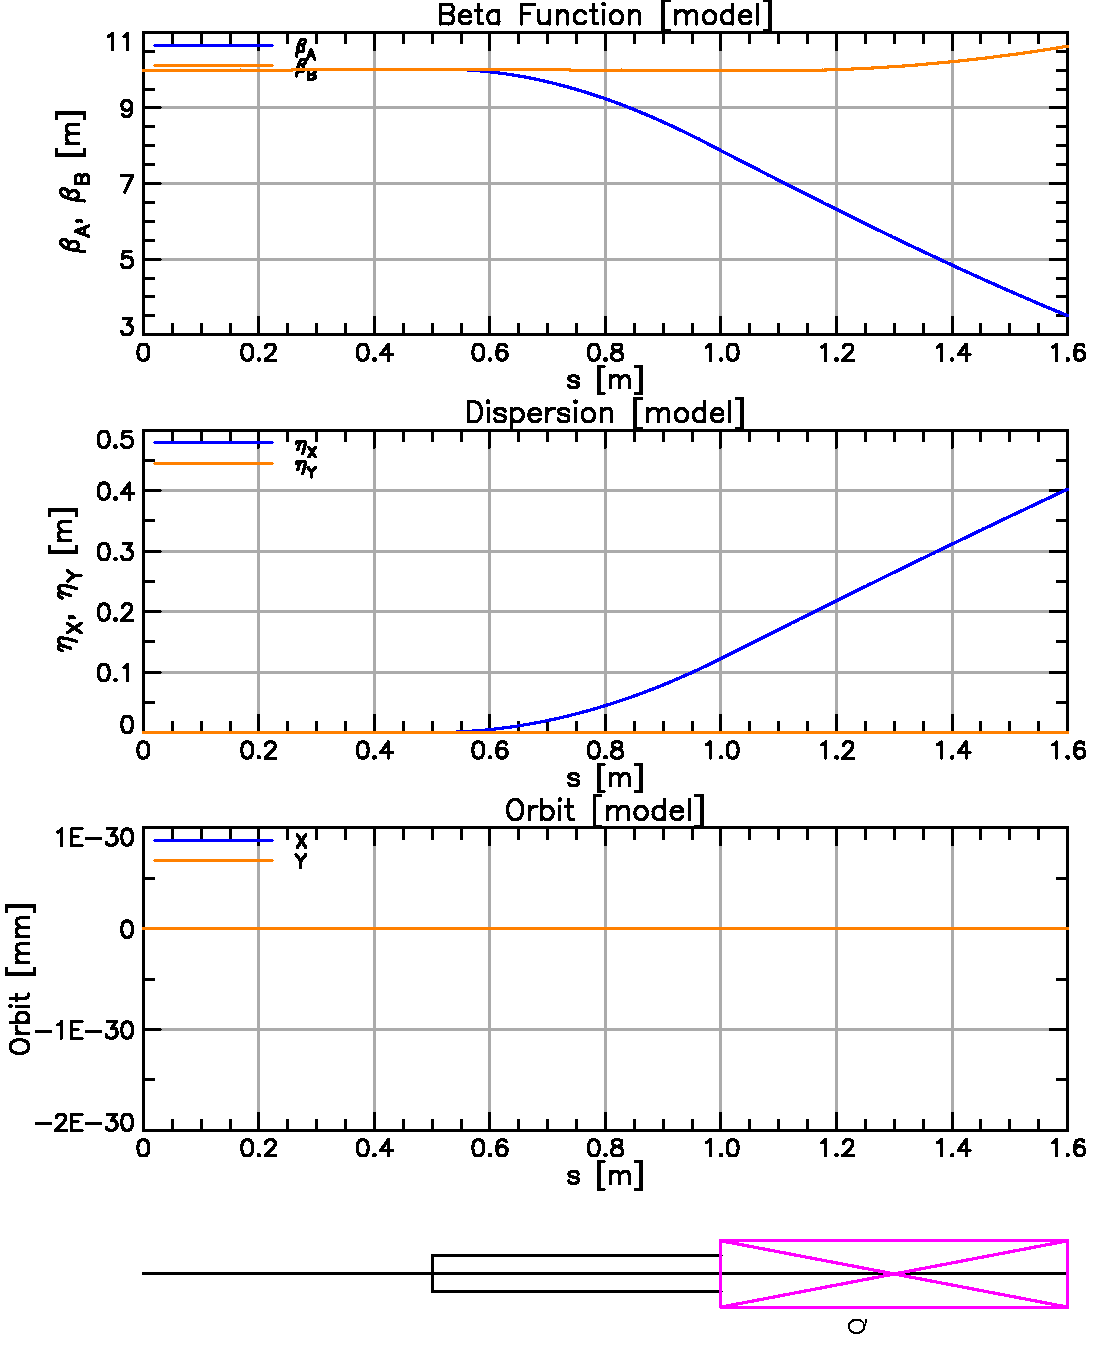
\includegraphics[width=\textwidth]{lat-init.pdf}
    \caption{Initial graphics when \tao is run with the \vn{lat.bmad} lattice file.}
    \label{f:lat.init}
  \end{subfigure}
  \hfil
  \begin{subfigure}[b]{0.47\textwidth}
    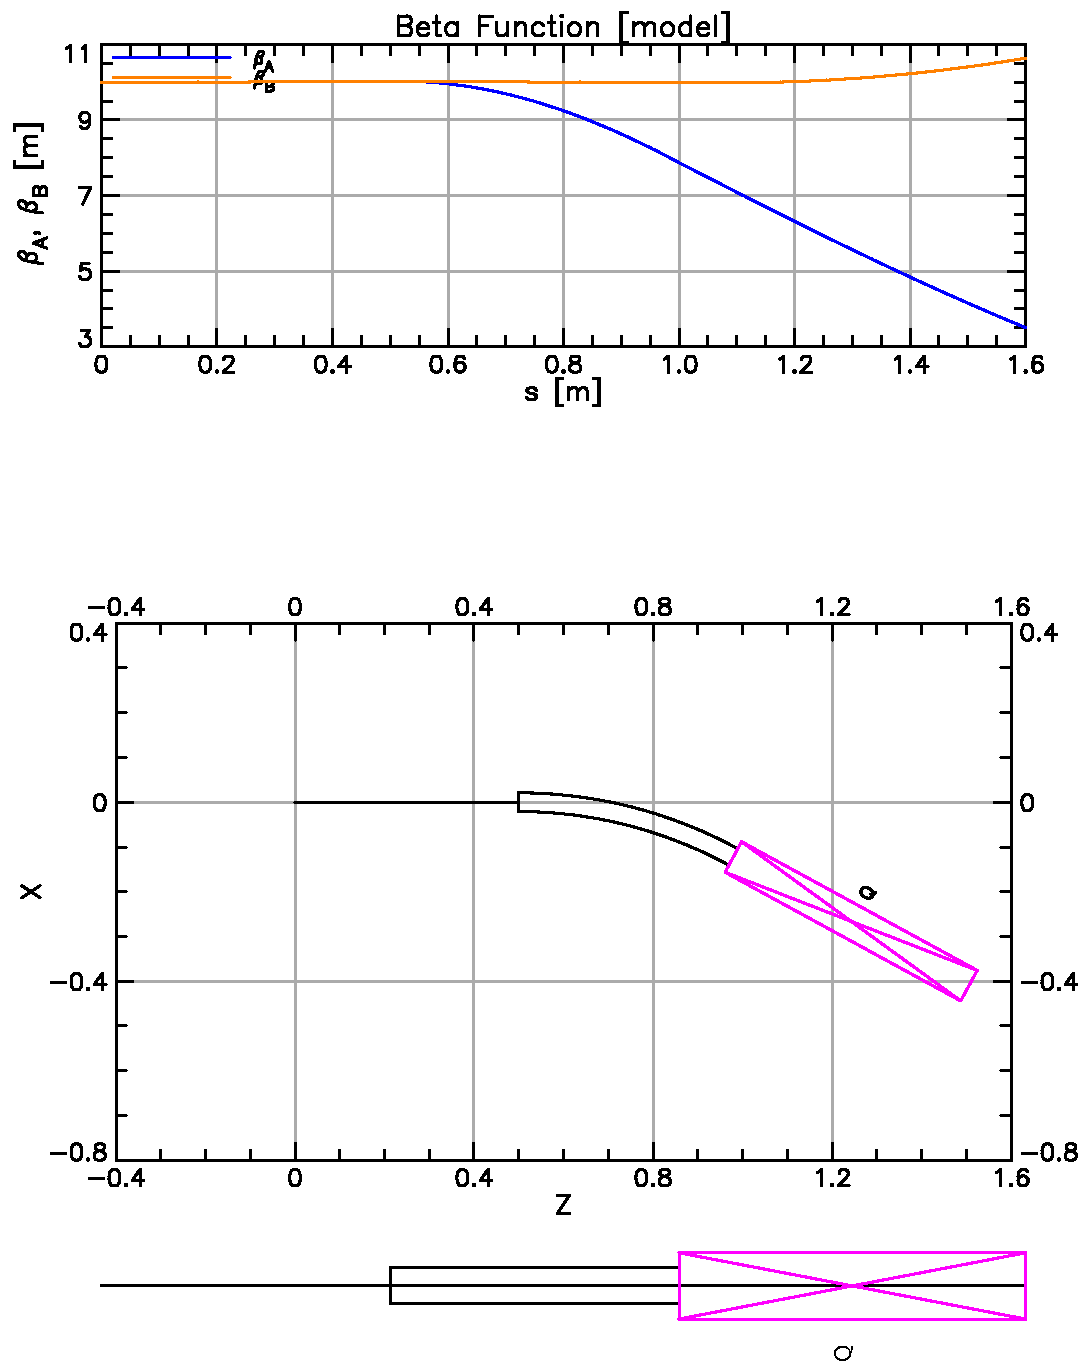
\includegraphics[width=\textwidth]{lat-floor.pdf}
    \caption{Graphics after a \vn{place r22 floor_plan} command.}
    \label{f:lat.floor}
  \end{subfigure}
  \caption{Example \tao graphics.}
\end{figure}

To run, \tao needs a lattice file as input.  Cutting and pasting from PDF is problematical so
instead the lattice files used in this tutorial are available for download from the web. Go to the
\bmad web site (\sref{s:resources}), Follow a link to either the \bmad or \tao manual and there
should be a further link to the lattice files. Alternatively, the lattices are available in any
\vn{Distribution} or \vn{Release} (\sref{s:orientation}) in the directory:
\begin{code}
examples/bmad_tao_tutorial_files/
\end{code}
Each lattice shown in this tutorial lists the appropriate file name on the first line.

Alternatively, you can use one of the more complicated lattices in the directory
\begin{code}
examples/lattice_file_examples
\end{code}


As an example of how to run \tao, the lattice file shown in section~\sref{s:bmad.intro} will be
used. This lattice file is named \vn{simple.bmad}.  Make sure that the directory from which you are
running \tao does not have a file called \vn{tao.init} since this file can affect things (more on
that later). Copy \vn{simple.bmad} to your working directory and run \tao with the command:
\begin{code}
> tao -lat simple.bmad
\end{code}
\tao should open a window for plotting as shown in Figure~\ref{f:lat.init}. If this window is too
large for your screen, you can adjust the size of the plotting window by using the \vn{-geometry}
option at startup. Example:
\begin{code}
> tao -lat simple.bmad -geom 400x400
\end{code}
Consult the \tao manual for a list of command line arguments or use the command:
\begin{code}
> tao -help
\end{code}

In your terminal window there should be a ``\vn{Tao>}'' prompt where you can type \tao commands.

%----------------------------------------------------------
\Section{Tao: Getting Help}

First: Start \tao as explained in section~\sref{s:tao.start} with the lattice file
\vn{simple.bmad}.

To get a list of Tao commands use the \vn{help} command:
\begin{code}
Tao> help

Type 'help <command>' for help on an individual command
Available commands:
  alias                             read
  call                              restore
  change                            reinitialize
  clip                              run_optimizer
  continue                          scale
  derivative                        set
  end_file                          show
  exit                              single_mode
  flatten                           spawn
... etc...
\end{code}

Note: For brevity's sake, ``\vn{... etc...}'' is used when the output has been truncated. Also the output shown
is sometimes modified to fit the printed page.

\tao commands are documented in the ``\vn{Tao Line Mode Commands}'' chapter of the \tao manual.
This same documentation can be displayed using the ``\vn{help <command>}'' command where
\vn{<command>} is the name of a command. Example:
\begin{code}
Tao> help set

The "set" command is used to set values for data,
variables, etc. Format:
  set beam_init {n@}<component> = <value>
  set beam_start {n@}<coordinate> = <value>
  set bmad_com <component> = <value>
  set csr_param <component> = <value>
  set curve <curve> <component> = <value>
  set data <data_name>|<component> = <value>
  set default <parameter> = <value>
  set element <element_list> <attribute> = <value>
  set floor_plan <component> = <value>
  set geodesic_lm <component> = <value>
... etc...

Also see the "change" command . The "change" command is specialized
for varying real parameters while the "set" command is more general.

... etc...

Use the command:
  help set <what>
to obtain more information on a particular set subtopic. Example:
  help set plot
\end{code}

Some commands are complicated enough so that there is a second help level. The \vn{set} command is
an example of such a command. Thus you can type \vn{help set curve} for help on setting plotting
curve parameters.

%----------------------------------------------------------
\Section{Tao Show Command}

Start \tao as explained in section~\sref{s:tao.start} with the lattice file
\vn{simple.bmad}

\subsection{To Show a List of Elements in the Lattice}

To show the elements in the lattice use the command \vn{show lattice}:
\begin{code}
 Tao> show lat
      Values at End of Element:
 Index  name      key                       s       l    beta     phi ...
                                                            a       a ...
     0  BEGINNING Beginning_Ele         0.000     ---   10.00   0.000 ...
     1  D         Drift                 0.500   0.500   10.03   0.050 ...
     2  B         Sbend                 1.000   0.500    7.87   0.104 ...
     3  Q         Quadrupole            1.600   0.600    3.50   0.217 ...
     4  END       Marker                1.600   0.000    3.50   0.217 ...
 Index  name      key                       s       l    beta     phi ...
                                                            a       a ...
      Values at End of Element:
\end{code}

Notice that \bmad adds two extra elements to the lattice. A zero length beginning element called \vn{BEGINNING}
and a zero length marker element at the end called \vn{END}.

The "show lat" command, like many other commands, has lots of optional parameters to customize the
table of information printed:

\begin{code}
Tao> help show lat

Syntax:
  show lattice {-0undef} {-all} {-attribute <attrib>} {-base}
      {-blank_replacement <string>}  {-branch <name_or_index>}
      {-custom <file_name>} {-design} {-floor_coords} {-lords} {-middle}
      {-no_label_lines} {-no_tail_lines} {-no_slaves} {-orbit} 
      {-remove_line_if_zero <column #>} {-s <s1>:<s2>} {-tracking_elements}
      {<element_list>}

Show a table of Twiss and orbit data, etc. at the specified element locations. 
The default is to show the parameters at the exit end of the elements. 
... etc...
\end{code}

%----------------------------------------------------------
\subsection{To Show the Attributes of a Lattice Element}

Use the \vn{show element} command to show the attributes of a particular lattice elements. Example:
\begin{code} 
Tao> show ele b   ! or: show ele 2

 Element #                2
 Element Name: B
 Key: Sbend
 Sub Key: SBend
 S_start, S:    0.500000,    1.000000
 Ref_time:  3.340005E-09

 Attribute values [Only non-zero/non-default values shown]:
    1   L                            =  5.0000000E-01 m
    6   G                            =  1.0000000E+00 1/m
    8   RHO                          =  1.0000000E+00 m
   13   SPIN_FRINGE_ON               =  T (1)
   19   E1                           =  0.0000000E+00 rad
   20   E2                           =  0.0000000E+00 rad
   29   L_SAGITTA                    =  3.1087578E-02 m
     ... etc...

Twiss at end of element:
                          A              B            Cbar    ...
  Beta (m)         7.87064432     9.99974729  |   0.00000000  ...
  Alpha            3.93634109     0.20027369  |   0.00000000  ...
  Gamma (1/m)      2.09573455     0.10401358  |   Gamma_c =   ...
  Phi (rad)        0.10395730     0.09991742            X     ...
  Eta (m)          0.12241744     0.00000000     0.12241744   ...
  Etap             0.48187421     0.00000000     0.48187421   ...

Orbit:  Positron   State: Alive
         Position[mm] Momentum[mrad]        Spin   |
  X:       0.00000000     0.00000000               | Particle [sec]: ...
  Y:       0.00000000     0.00000000               | Part-Ref [sec]: ...
  Z:       0.00000000     0.00000000               | (Ref-Part)*Vel  ...
\end{code}
Note: By default, only non-zero attributes are shown. Use the -all option to see all the attributes.

%----------------------------------------------------------
\subsection{To Show a List of Elements Using Wild Cards}

Use the \vn{show element} with a wild card character to show all elements matching a particular
pattern. Wild card character are:
\begin{code}
"*" -- Matches to any number of characters.
"%" -- Matches to any single character.
\end{code}
The general syntax is:
\begin{code}
show element <element_type>::<name_with_wild_card_characters>
\end{code}

For example, to show all elements whose name begins with "Q" the command is:
\begin{code}
Tao> show ele q*

         1  Q                                                1.000
Number of Matches: 1
\end{code}

Or to show all sbend elements the command is:
\begin{code}  
Tao> show ele sbend::*

         2  B                                                2.000
Number of Matches: 1
\end{code}

%----------------------------------------------------------
\Section{Introduction to Plotting in Tao}

\vn{To Do}: Start \tao as explained in section~\sref{s:tao.start} with the lattice file
\vn{simple.bmad} of section~\sref{s:bmad.intro} and experiment with the plotting as shown 
in this section.

The default is to have three plots: beta, dispersion, and
orbit, along with what is called a \vn{lat_layout} plot (at the bottom of the window) that
graphically shows the lattice elements. Note: If you do not want \tao to display the plot window,
use the \vn{-noplot} option on the command line.

%----------------------------------------------------------
\subsection{Plot Page Parameters}

\begin{figure}[tb]
  \centering
  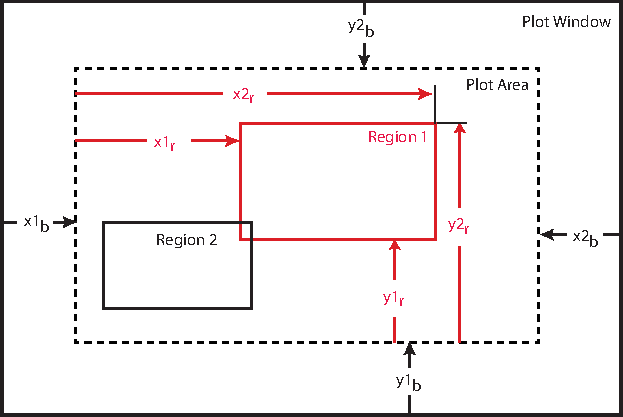
\includegraphics[width=0.7\textwidth]{plot-page.pdf}
  \caption{The plot window is divided up into a number of rectangular \vn{regions} into
which a plot \vn{template} can be placed. Regions can overlap.}
  \label{f:plot.regions}
\end{figure}

The plot window has a number of parameters that can be displayed using the \vn{show plot}
command:

\begin{code}
Tao> show plot
plot_page parameters:
  %size                         = 500     600
  %n_curve_pts                  = 401
  %text_height                  = 12.000
... etc...

Templates:
   Plot                                    Description
   ----------------------------            -------------------
   alpha                                   Twiss alpha function
   b_div_curl                              Magnetic Field Divergence and Curl.
   b_field                                 Magnetic Field Along Orbit
   beta                                    Twiss beta function
   bunch_sigma_xy                          Bunch transverse sigmas
   bunch_R1_R2                             Bunch phase space plot.
   cbar                                    Cbar coupling matrix
   dbeta                                   Chromatic normalized beta beat
... etc...

                                               Location on Page
Plot Region         <-->  Plot                 x1    x2    y1    y2
-----------               -----------------------------------------
layout              <-->  lat_layout          0.00  1.00  0.00  0.15
r11                 <-->                      0.00  1.00  0.15  1.00
r12                 <-->                      0.00  1.00  0.58  1.00
r22                 <-->                      0.00  1.00  0.15  0.58
r13                 <-->  beta                0.00  1.00  0.72  1.00
r23                 <-->  dispersion          0.00  1.00  0.43  0.72
r33                 <-->  orbit               0.00  1.00  0.15  0.43
r14                 <-->                      0.00  1.00  0.79  1.00
... etc...
\end{code}
The output of the \vn{show plot} is divided into three sections. The top section
shows some parameters like the size of the plot window. Use the \vn{set plot_page}
command to change these parameters. 

The middle section of the output of the \vn{show plot} command shows plot \vn{templates}.
Plot templates specify parameters for drawing plot. For example, how many graphs are
associated with a plot (in the plots of Figure.~\ref{f:lat.init} there are one graph per plot)
and how many curves per graph there are. \tao defines a set of default templates and custom
ones can be defined by constructing the appropriate initialization file. Directions for
constructing templates are given in the \vn{Initializing Plotting} section of the \vn{Tao
Initialization} chapter of the \tao manual.

The bottom section of the output of the \vn{show plot} command shows the plot \vn{regions} of the
plot window along with associated plots. The plot regions are rectangular regions of the plot window
into which a plot can be placed as illustrated in Figure~\ref{f:plot.regions}.  See the
\vn{Initializing Plotting} section of the \vn{Tao Initialization} chapter of the \tao manual. for
more details. With the present example, there are four regions that have plot. The \vn{r13} region
has a \vn{beta} plot, etc.


%----------------------------------------------------------
\subsection{Placing Plots}

The \vn{place} command is used to place a \vn{template} plot into a plot region. Example:
\begin{code}
Tao> place r22 floor_plan
\end{code}
This places a \vn{floor_plan} plot in the \vn{r22} region.
The result is shown in Figure~\ref{f:lat.floor}. Plots associated with other regions
that overlap the region that is used in the \vn{place} command are erased. 

Example place commands:
\begin{code}
Tao> place r22 none    ! Clear a region
Tao> place * none      ! Clear all regions
\end{code}

%----------------------------------------------------------
\subsection{Scaling Plots}

Plots can be scalled vertically using the \vn{scale} command:
\begin{code}
Tao> scale beta 0 20  ! Set y_min = 0, y_max = 20
Tao> scale r22 0 20   ! Same as above if beta plot in r22 region
Tao> scale beta       ! Tao will calculate nice bounds
Tao> scale all        ! "all" = all plots
Tao> scale            ! Same as "scale all"
\end{code}

The \vn{x_scale} command can be used to scale the horizontal axis and
the \vn{xy_scale} command can be used to simultaneously scale the x and y axis.
\begin{code}
Tao> x_scale beta 0.8 1.0   ! Scale horizontal axis
Tao> xy_scale floor_plan    ! Combined scale and x_scale.
\end{code}

\newpage

%----------------------------------------------------------
\Section{Model Design and Base Lattices in Tao}

When \tao runs, \tao instantiates three lattices:
\begin{description}
\item[Design Lattice] \Newline
The \vn{design} lattice corresponds to the lattice read in from the lattice
description file(s). Parameters of this lattice are never varied.
\item[Model Lattice] \Newline
Initially, when Tao is started, \vn{model} = \vn{design}. Essentially all commands to vary lattice
parameters vary parameters of this lattice.
\item[Base Lattice] \Newline
The \vn{base} lattice is a reference lattice used so that changes in the \vn{Model} 
lattice may more easily be viewed.
\end{description}

[Technically, \tao instantiates three lattices per \vn{universe}. See below.]

%----------------------------------------------------------
\subsection{Setup}

The lattice used to illustrate things in this section is:
\begin{code}
beginning[beta_a] = 10.   ! m
beginning[beta_b] = 10.   ! m
beginning[e_tot] = 10e6   ! eV
parameter[geometry] = open  ! or closed

d: drift, L = 0.5
b: sbend, L = 0.5, g = 1, e1 = 0.01, e2 = 0.02, g_err = 0.001
q: quadrupole, L = 0.6, k1 = 0.23

lat: line = (d, b, q)
use, lat
\end{code}

Copy this lattice to a file and run \tao with this lattice as explained in section~\sref{s:tao.start}.

\begin{figure}[tb]
  \centering
  \begin{subfigure}[b]{0.47\textwidth}
    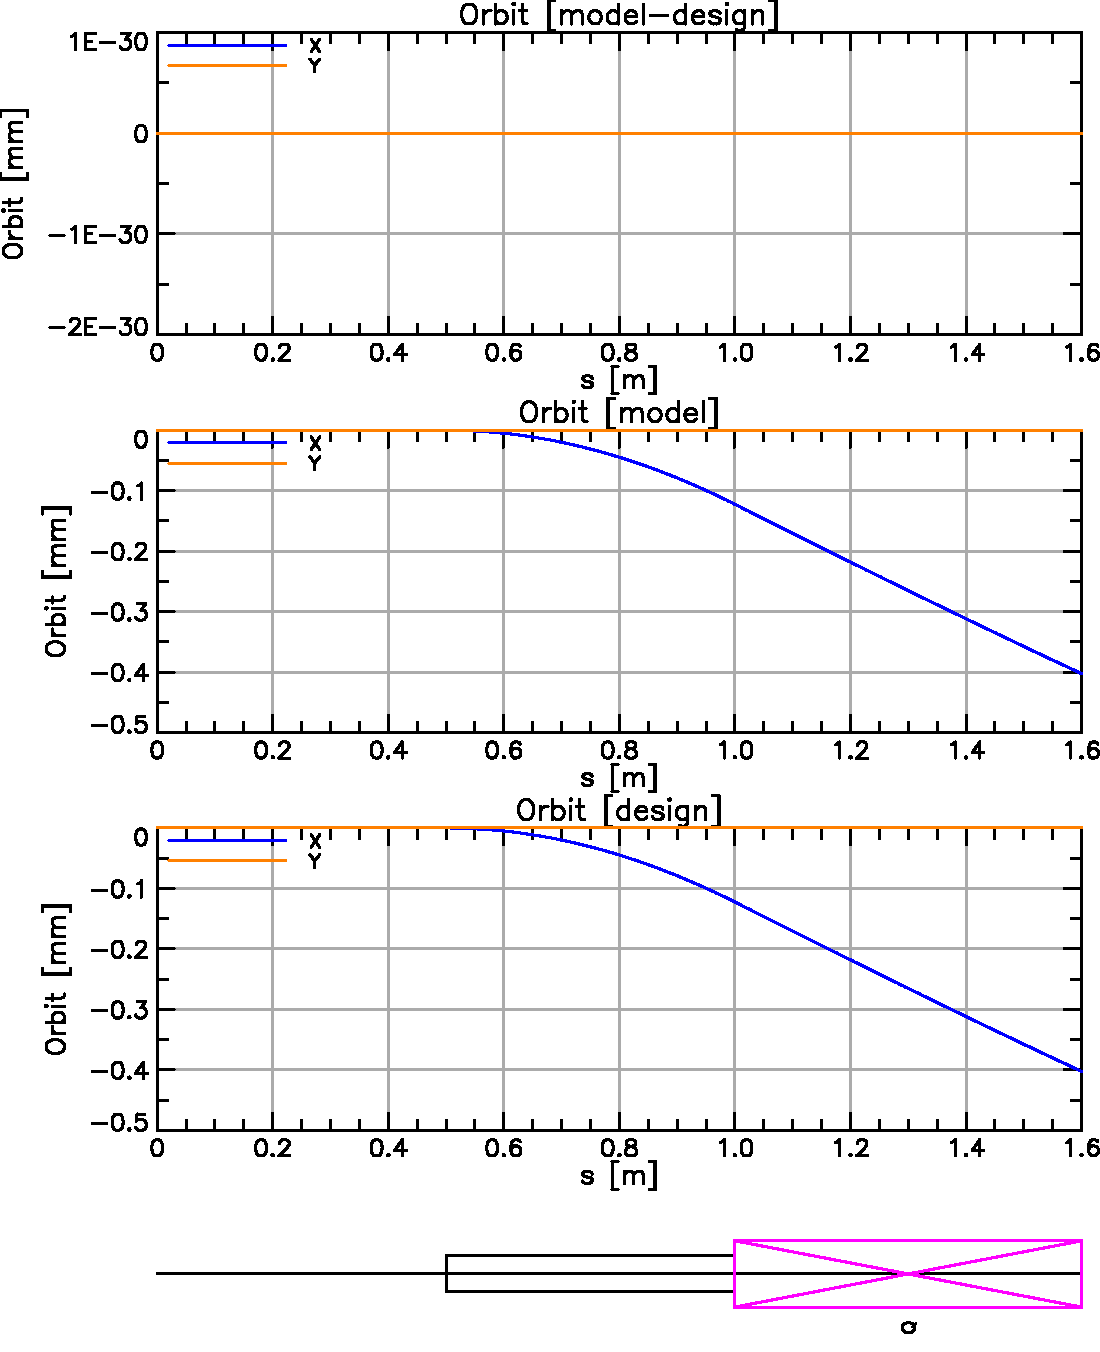
\includegraphics[width=\textwidth]{model-equal-design.pdf}
    \caption{Initially, the \vn{model} lattice and the \vn{design} lattices are the same.}
    \label{f:model.eq.design}
  \end{subfigure}
  \hfil
  \begin{subfigure}[b]{0.47\textwidth}
    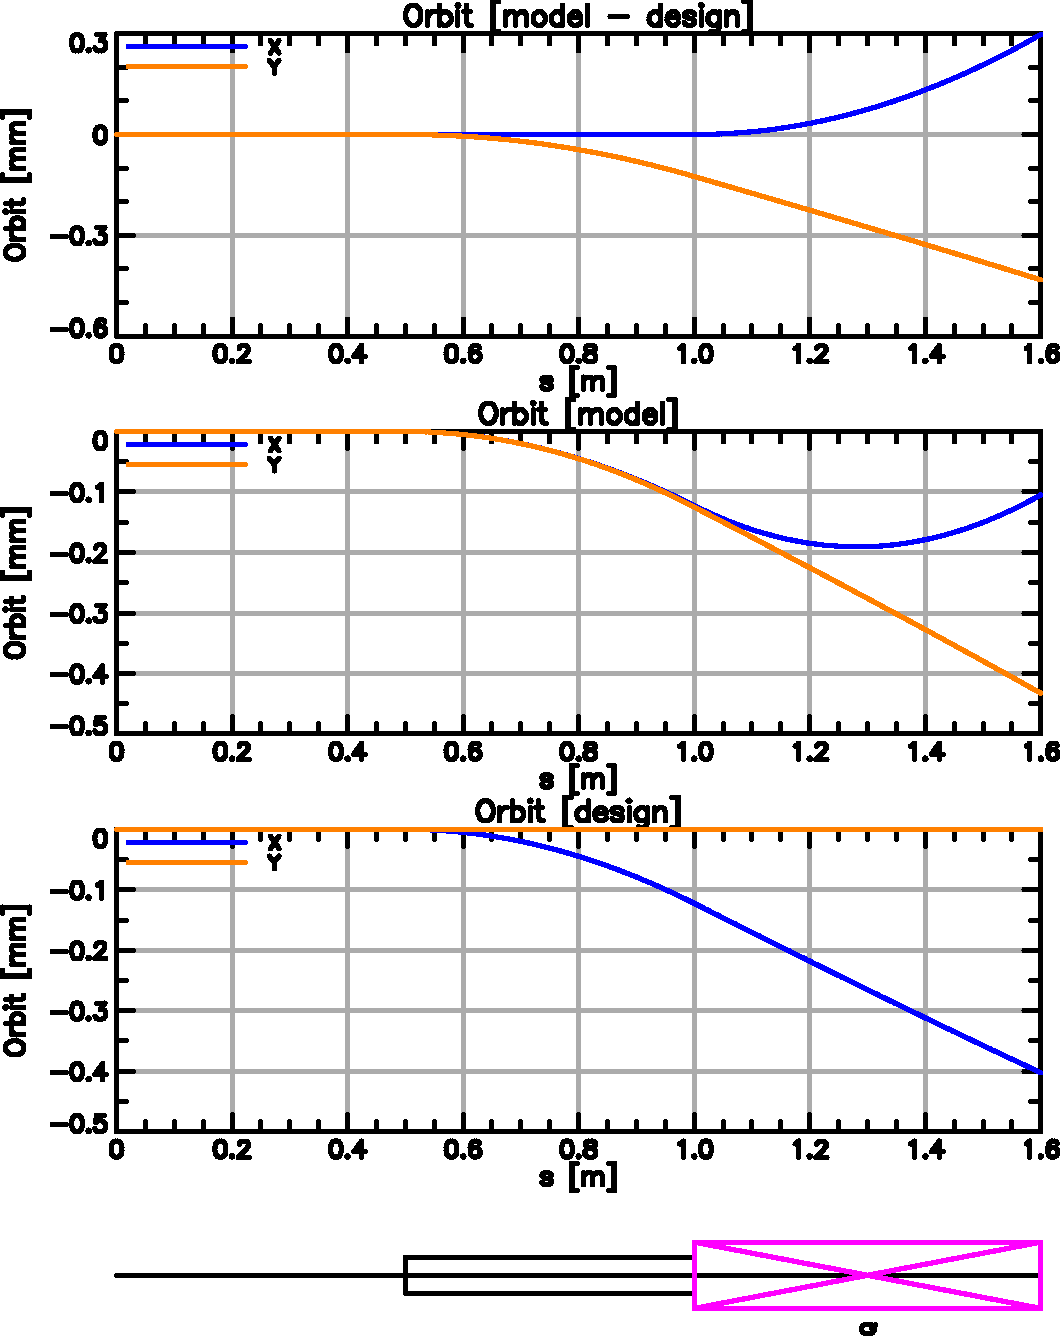
\includegraphics[width=\textwidth]{changed-model.pdf}
    \caption{The \vn{set} and \vn{change} commands will modify \vn{model} lattice parameters.}
    \label{f:changed.model}
  \end{subfigure}
  \caption{}
\end{figure}

%----------------------------------------------------------
\subsection{Changing Model Parameters}

To see the difference between the \vn{model} and \vn{design} lattices issue the following commands:
\begin{code}
Tao> place r23 orbit
Tao> place r13 orbit
Tao> set plot r33 component = design
Tao> set plot r13 component = model - design
Tao> scale
\end{code}
The result is shown in Figure~\ref{f:model.eq.design}. The bottom plot shows the \vn{design} lattice
orbit, the middle plot shows the \vn{model} lattice orbit and the top plot shows the difference in
orbits between \vn{model} and \vn{design}. Since the two lattices are the same when \tao is started,
the difference orbit is zero.

Now change the \vn{model} lattice using the following commands:
\begin{code}
Tao> change element b vkick  -0.0005   ! Changes by a given delta
Tao> set element q hkick = 0.001       ! Can be used with integers or logicals
Tao> scale
\end{code}
The \vn{change} command changes real numbers by a given delta. The \vn{set} command can be use with
parameters other than real numbers.  The result is shown in Figure~\ref{f:changed.model}. Since now
the \vn{model} lattice is not the same as the \vn{design} lattice the difference orbit is non-zero.

\begin{figure}[tb]
  \centering
  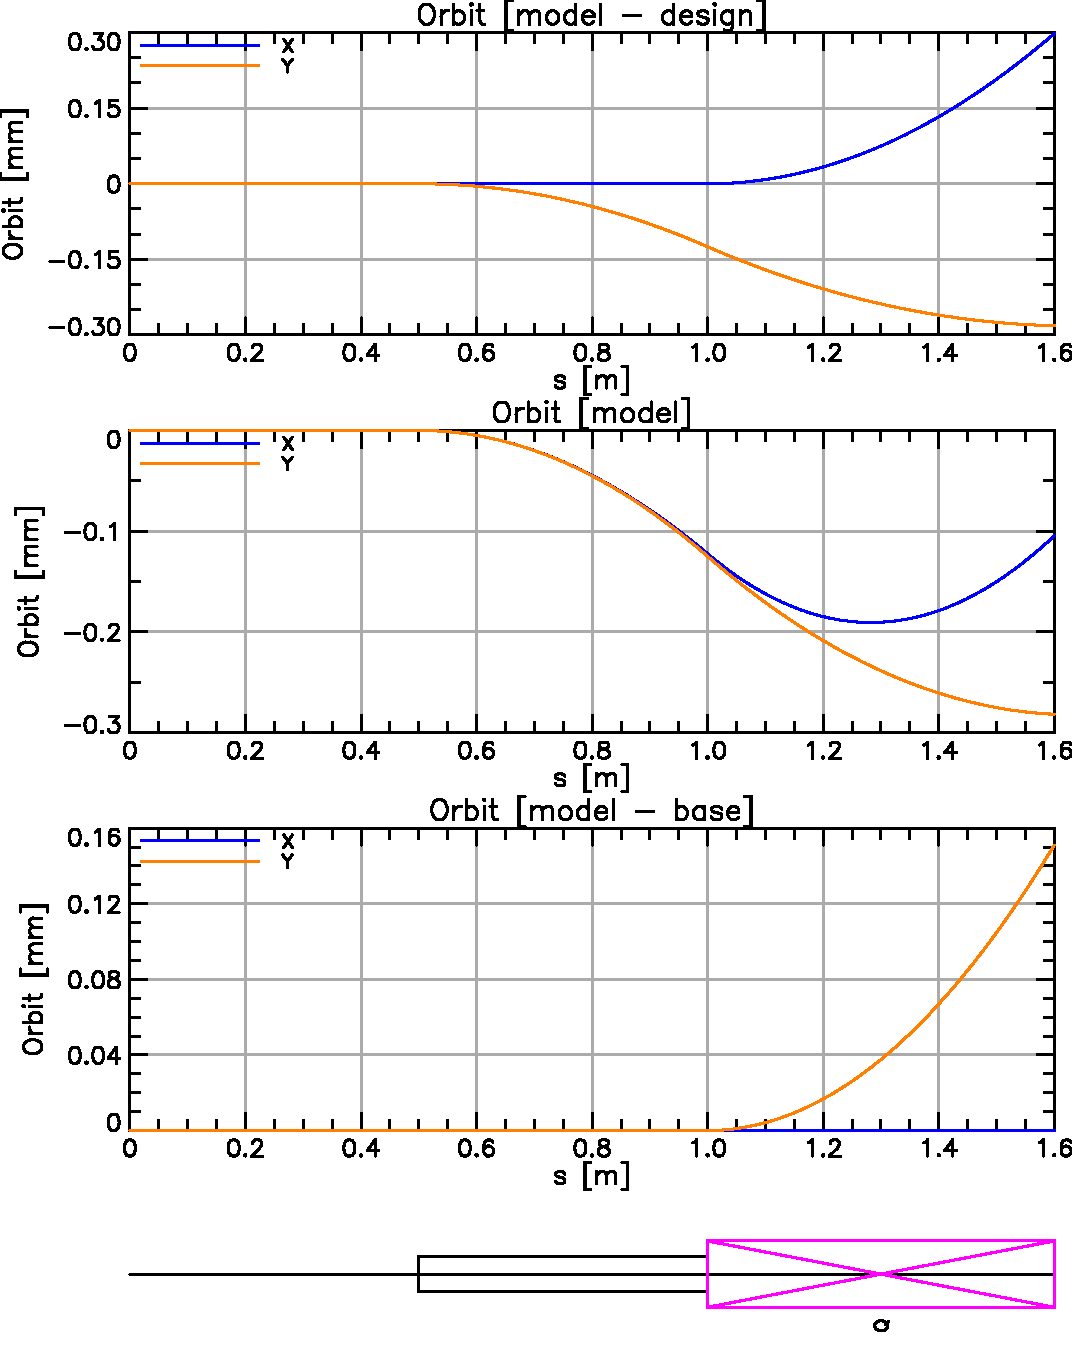
\includegraphics[width=0.7\textwidth]{with-base.pdf}
  \caption{The \vn{base} lattice is used to view changes when the reference lattice configuration
does not correspond to the \vn{design} lattice.}
  \label{f:base}
\end{figure}

%----------------------------------------------------------
\subsection{Using the Base Lattice}

The \vn{base} lattice is used to view changes when the reference lattice configuration does not
correspond to the \vn{design} lattice.

Continuing from the previous subsection, issue the following commands:
\begin{code}
Tao> set lattice base = model  ! Set the Base lattice = Model lattice.
Tao> set plot r33 component = model - base
Tao> set ele q vkick = 5e-4
Tao> scale
\end{code} 
The \vn{set lattice} command sets the \vn{base} lattice equal to the \vn{model}
lattice. The third command varies the \vn{model} lattice.  The result is shown in
Figure~\ref{f:base}. The bottom plot of the orbit difference between \vn{model} and
\vn{base} is not the same as the orbit difference between \vn{model} and \vn{design}.

%----------------------------------------------------------
\subsection{Multiple Universes}

\tao has a concept called a \vn{universe}. A \vn{universe} consists of \vn{model}, \vn{design},
and \vn{base} lattice along with a \vn{data} which can, say, represent something like
an orbit measurement. In \tao multiple universes may be defined. This is useful in a number of 
situations. For example, if multiple orbit measurements have been made with steering magnets
changing between measurements, each measurement could be associated with a different universe
and the entire collection of measurements could be analyzed simultaneously. 

The discussion of multiple universes is beyound this tutorial and the interested reader is 
referred to the \tao manual.


%----------------------------------------------------------
\Section{Control Elements}

%----------------------------------------------------------
\subsection{Overview}

Control elements are elements that control the parameters of other elements. There are three types
of control elements called \vn{groups}, \vn{overlays}, and \vn{girders}. \vn{Groups} and
\vn{overlays} are convenient to do such things as simulate control room "knobs". For example a power
supply that powers a chain of magnets can be simulated with a control element.
\vn{Girder} elements are used for simulating support structures that support lattice elements.

Note: \vn{Group}, \vn{overlay}, and \vn{girder} elements are known as \vn{minor} lords since they
only control a subset of an element's attributes. The other type of lord elements, \vn{multipass}
and \vn{super} lords, are called \vn{major} lords.

%----------------------------------------------------------
\subsection{Example Lattice}


The lattice used to illustrate control elements is:
\begin{code}
beginning[beta_a] = 10
beginning[beta_b] = 10

parameter[particle] = muon
parameter[p0c] = 1e9
parameter[geometry] = open

q: quadrupole, l = 1
b: sbend, l = 1
ll: line = (q, b)
use, ll

ov1: overlay = {q[k1]: a+b^2, b[g]: 0.1*a+tan(b)}, var = {a, b}
ov2: overlay = {q[k1]: 0.7, q[x_offset]: 0.1*kt}, var={kt}
gr1: group = {b[e1]: 0.4*sqrt(k)}, var = {k}
\end{code}

Explanation:
\begin{itemize}
\item
The overlay \vn{ov1} controls two parameters: 
The \vn{k1} attribute of element \vn{q} (denoted \vn{q[k1]}) and the \vn{g} attribute of element
\vn{b} (denoted \vn{b[g]}.
\item
Overlay \vn{ov1} has two variables called \vn{a} and \vn{b} that are used to control the two attributes.
\item
The formulas for overlay \vn{ov1} that are used to calculate the the values of the two controlled
attributes are \vn{a+b$^2$} for \vn{q[k1]} and \vn{0.1*a+tan(b)} for \vn{b[g]}.
\item 
Since overlay \vn{ov2} also controls \vn{q[k1]}, the value of \vn{q[k1]} is the sum of the
contributions of \vn{ov1} and \vn{ov2}.
\item
The given "formula" for the control of \vn{q[k1]} by \vn{ov2} is just a constant: 0.7. 
This is a shorthand notation and the actual formula used is \vn{0.7*kt}. 
Note: When this shorthand notation is used, only one variable (in this case \vn{kt}) may be used by the overlay.
\item
The difference between \vn{group} and \vn{overlay} elements is explained below.
\end{itemize}

%----------------------------------------------------------
\subsection{Control Element Organization in the Lattice}

Copy the above lattice to a file and run \tao with this lattice as explained in
section~\sref{s:tao.start}.

To see the elements in the lattice use the \vn{show lattice} command:
\begin{code}
Tao> show lat

      Values at End of Element:
 Index  name      key                       s       l    beta     phi ...
                                                            a       a ...
     0  BEGINNING Beginning_Ele         0.000     ---   10.00   0.000 ...
     1  Q         Quadrupole            1.000   1.000   10.10   0.100 ...
     2  B         Sbend                 2.000   1.000   10.40   0.197 ...
     3  END       Marker                2.000   0.000   10.40   0.197 ...
Lord Elements:
     4  OV1       Overlay               2.000     ---   10.40   0.197 ...
     5  OV2       Overlay               1.000     ---   10.10   0.100 ...
     6  GR1       Group                 2.000     ---   10.40   0.197 ...
 Index  name      key                       s       l    beta     phi ...
                                                            a       a ...
      Values at End of Element:
\end{code}

The list of lattice elements is divided up into two sections
\begin{itemize}
\item
The \vn{"tracking"} part of the lattice are the elements to be tracked through. Here the tracking part of
the lattice is elements 0 through 3.
\item
The \vn{"lord"} section of the lattice are where the overlay and group elements (and other "lord"
elements as described elsewhere). Here the lord section is elements 4 through 6.
\end{itemize}

%----------------------------------------------------------
\subsection{Examining Controls}

To see how things are controlled, use the \vn{show element} command. For example:
\begin{code}
Tao> show ele 4

 Element #                4
 Element Name: OV1
 Key: Overlay
... ... ... etc...
Slave_status: Free
Lord_status:  Overlay_Lord
Control Variables:
    1   A                                         =  0.0000000E+00
    2   B                                         =  0.0000000E+00
Slaves: [Attrib_Val = Expression_Val summed over all controlling overlays.]
   Index   Ele_Name  Attribute   Attrib_Value  Expression_Val    Expression
       1   Q         K1            0.0000E+00      0.0000E+00    a+b^2
       2   B         G             0.0000E+00      0.0000E+00    0.1*a+tan(b)
... ... ... etc...
\end{code}

And

\begin{code}
Tao> show ele q
 Element #                1
 Element Name: Q

        ... etc...

Slave_status: Minor_Slave
Controller Lord(s):
   Index   Name        Attribute           Lord_Type           Expression
       4   OV1         K1                  Overlay             a+b^2
       5   OV2         K1                  Overlay             0.7*KT
       5   OV2         X_OFFSET            Overlay             0.1*kT

Lord_status:  Not_a_Lord

        ... etc...
\end{code}

%----------------------------------------------------------
\subsection{Overlay Control}

When a element parameter is controlled by one or more overlays, the value of the element parameter
is the sum of the values for each overlay.

In this case there are two overlays controlling the \vn{q[k1]} attribute:
\begin{code}
Tao> set ele ov1 a = 0.02
Tao> set ele ov2 kt = 0.01

Tao> show ele q
 Element #                1
 Element Name: Q
... etc...

 Attribute values [Only non-zero/non-default values shown]:
    1   L                            =  1.0000000E+00 m
    4   K1                           =  2.7000000E-02 1/m^2
... etc...
\end{code}
The value of \vn{q[k1]} is 0.027 = .02 (from \vn{ov1}) + 0.007 (from \vn{ov2}).

The value of a parameter that is controlled by overlays may not be directly changed:
\begin{code}
Tao> set ele q k1 = 0.02
[ERROR | 2017-AUG-26 13:29:26] attribute_free:
    THE ATTRIBUTE: K1
    OF THE ELEMENT: Q
    IS NOT FREE TO VARY SINCE:
    IT IS CONTROLLED BY THE OVERLAY: OV1
\end{code}

%----------------------------------------------------------
\subsection{Group Control}

Group Control

Unlike overlay control, a parameter that is controlled by one or more group elements is free to vary.
When a group element is varied, a change in the value for parameters it controls is computed.
Consider \vn{group} element \vn{gr1}:
\begin{code} 
Tao> set ele gr1 k = 0.01

Tao> show ele gr1
 Element #                6
 Element Name: GR1
 Key: Group

... etc...    

Slave_status: Free
Lord_status:  Group_Lord
Control Variables:
    1   K  =  1.0000000E-02           OLD_K  =  1.0000000E-02
Slaves:
   Index   Ele_Name  Attribute   Attrib_Value  Expression_Val    Expression
       2   B         K1            4.0000E-02      4.0000E-02    0.4*sqrt(k)
\end{code}
A \vn{group} element not only has associated variables (in this case a single variable \vn{k}) but
\bmad also keeps a record of what is called the ``old'' value (\vn{old_k}). When the above \vn{set
  ele gr1} command is executed, the value of \vn{gr1[k]} becomes 0.01. \bmad detects that \vn{k}
and \vn{old_k} are different and
\begin{enumerate}
\item
Evaluates the difference \vn{0.4*sqrt(k)} - \vn{0.4*sqrt(old_k)} = 0.04
\item
Increments the value of \vn{b[k1]} by 0.04.
\item
Sets the value of \vn{old_k} equal to \vn{k}.
\end{enumerate}
Since the old value of \vn{b[k1]} was zero. The new value of \vn{b[k1]} is 0.04

Now consider the effect of the following two set commands:
\begin{code}
Tao> set ele b k1 = 0.02
Tao> set ele gr1 k = 0.04

Tao> show ele gr1
... etc...
Control Variables:
    1   K  =  4.0000000E-02           OLD_K  =  4.0000000E-02
Slaves:
   Index   Ele_Name  Attribute   Attrib_Value  Expression_Val    Expression
       2   B         K1            6.0000E-02      8.0000E-02    0.4*sqrt(k)
\end{code}
The \vn{set ele b} command sets the value of \vn{b[k1]} to 0.02 and the \vn{set ele gr1} command
sets the value of \vn{gr1[k]} to 0.04 which causes the value of \vn{b[k1]} to increase by 0.04 (=
0.08 - 0.04) from 0.02 to a value of 0.06.

What is a group element useful for? Example: Consider the situation where you want to control the
chromaticity (change in tune with particle energy) of a ring by varying sextupole strengths. To
change the chromaticity by 1 unit you want to change the sextupole strengths by some amount that you
compute. Here you don't care about the value of the sextupole strengths, you only want to vary the
sextupole strengths by a delta.

\begin{code} 
raw_xqune_1 : group ={SEX_08W:-.6415E-03*k2,...}, var = {k2}
\end{code}

Notes:
\begin{itemize}
\item
Group and overlay elements can control other group and overlay elements.
\item
A given element parameter may only be controlled by a set of group elements or a set of overlay
elements but may not be controlled by both group and overlay elements.
\end{itemize}

%----------------------------------------------------------
\subsection{Girders}

A third type of controller is the \vn{girder} element which can be used to simulate support
structures. See the Bmad manual for more details.

\newpage

%----------------------------------------------------------
\Section{Machine Coordinates and Patch Elements}

This section describes the coordinate systems used to describe the positioning
of lattice elements.

\begin{figure}[tb]
  \centering
  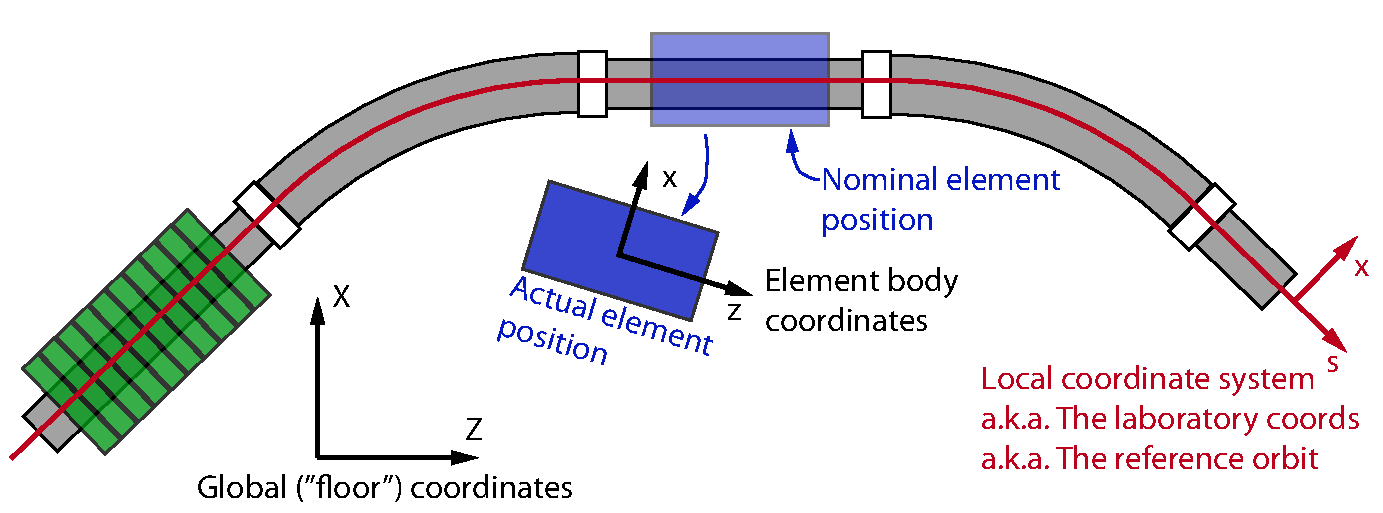
\includegraphics[width=0.9\textwidth]{coordinates.pdf}
  \caption{The three coordinate systems used to describe lattice element positioning:
\vn{Global}, \vn{reference}, and \vn{element body} coordinates.}
  \label{f:coordinates}
\end{figure}

%----------------------------------------------------------
\subsection{Coordinate Systems}

There are three coordinate systems that are used to describe the positioning
of lattice elements as shown in Figure~\ref{f:coordinates}:
\begin{description}
\item[Glorbal Coordinates] \Newline
The \vn{global} (also called \vn{floor}) coordinate system is independent of the accelerator and is 
"attached" to the building the accelerator is in. Typically, the Y-axis is taken to be pointing vertically up
and (X, Z) is the horizontal plane.
\item[Reference Coordinates] \Newline
The \vn{global} coordinate system is not convenient for describing where particles are as they move
through the lattice. For this the \vn{local} (also called \vn{laboratory}, also called \vn{reference}) curvilinear coordinate 
system is used to describe particle positions and also to describe the nominal position of the
lattice elements.

Traveling on the \vn{s} curve of the local coordinate system there is imagined to be a \vn{reference particle}.
Frequently, this reference particle is thought of as describing the center of a bunch of particles.
\item[Element Body Coordinates] \Newline
Elements can be shifted from their nominal position ("misalignments"). So to describe things like
electric and magnetic fields or apertures (which depend upon the elements actual position),
\vn{element body} coordinates are used. 
The \vn{element body} coordinates are the coordinates attached to the physical element. Without any "misalignments",
the \vn{element} coordinates correspond to the \vn{laboratory} coordinates.
\end{description}

\begin{figure}[tb]
  \centering
  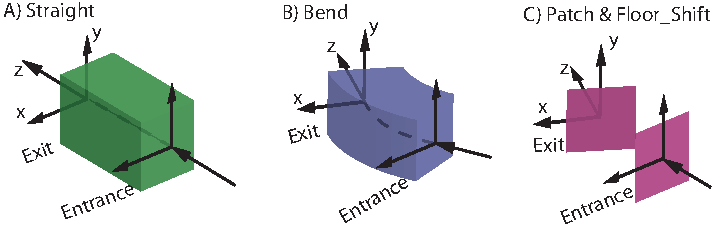
\includegraphics[width=0.9\textwidth]{element-coord-frame.pdf}
  \caption{Lattice element geometry types: \vn{Straight}, \vn{bend}, and \vn{patch}.}
  \label{f:body.types}
\end{figure}

%----------------------------------------------------------
\subsection{Element Geometry Types}

All lattice elements have an ``\vn{entrance}'' end and an ``\vn{exit}'' end. Normally a particle
will enter the element at the \vn{entrance} end and exit at the \vn{exit} end but this is not always
true.

All elements in \bmad have one of three geometry types as shown in Figure~\ref{f:body.types}.  These
three types are called \vn{straight}, \vn{bend} and \vn{patch} based upon how the element body
coordinates transform as a function of the longitudinal \vn{s} position from the \vn{entrance} end
of the element to the \vn{exit} end.
\begin{description}
\item[Straight Geometry] \Newline
With \vn{straight} elements like \vn{drift}s and \vn{quadrupole}s, the element body coordinates
transform as a translation along the \vn{entrance} \vn{z}-axis so that the \vn{exit} coordinates are
co-linear with the \vn{entrance} coordinates.
\item[Bend Geometry] \Newline
(\vn{Sbend} and \vn{rbend}) elements have a \vn{bend} geometry where the body coordinates rotate
about an axis which is in the $x$-$y$ plane of the \vn{entrance} (and \vn{exit}) coordinates.
\item[Patch Geometry] \Newline 
\vn{Patch} and \vn{floor_shift} elements have a \vn{patch} geometry where the exit coordinates can
be arbitrarily positioned with respect to the entrance coordinates (see below).
\end{description}

%----------------------------------------------------------
\subsection{Local Coordinate System Construction}

\begin{figure}[tb]
  \centering
  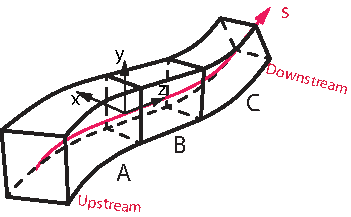
\includegraphics[width=0.6\textwidth]{element-stream.pdf}
  \caption{The \vn{local} coordinate system is constructed by taking the ordered list of lattice elements and
connecting the \vn{exit} frame of one element to the \vn{entrance} frame of the next.}
  \label{f:leggo}
\end{figure}

The \vn{local} coordinate system is constructed by taking the ordered list of lattice elements and
connecting the \vn{exit} frame of one element to the \vn{entrance} frame of the next (just like LEGO
blocks). Given a line constructed as:
\begin{code}
    lat: line = (A, B, C)
\end{code}
The result could look as shown in Figure~\ref{f:leggo}.

%----------------------------------------------------------
\subsection{Laboratory Coordinates Relative to Global Coordinates}

\begin{figure}[tb]
  \centering
  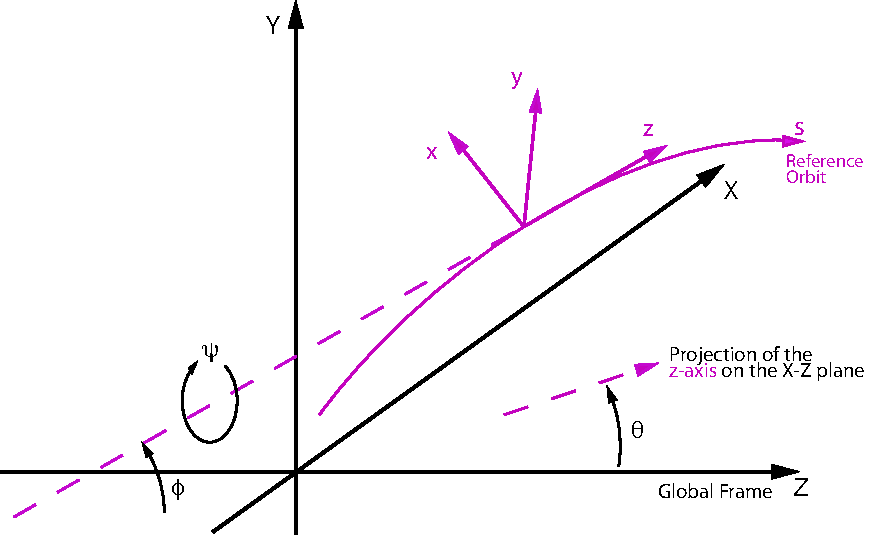
\includegraphics[width=0.9\textwidth]{global-coords.pdf}
  \caption{The global coordinate system.}
  \label{f:global}
\end{figure}

For any given position on the reference orbit, the \vn{local} coordinate system is described with
respect to the \vn{global} coordinate system by 6 parameters as shown in Figure~\ref{f:global}:
\begin{itemize}
\item (\vn{X}, \vn{Y}, \vn{Z}) global position
\item \vn{$\theta$} azimuth angle in the (X, Z) plane.
\item \vn{$\phi$} elevation angle
\item \vn{$\psi$} roll angle.
\end{itemize}

Notes:
\begin{itemize}
\item The default is for the beginning of the lattice (\vn{s} = 0) is to have the local (x, y, z) aligned with the 
global (X, Y, Z).
\item For a machine that lies in the horizontal plane, \vn{$\phi$} and \vn{$\psi$} angles are zero.
\end{itemize}


%----------------------------------------------------------
\subsection{Element Misalignments}


\begin{figure}[tb]
  \centering
  \begin{subfigure}[b]{0.62\textwidth}
    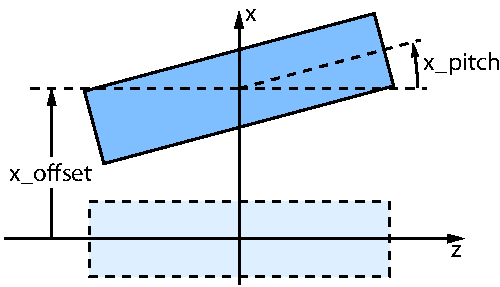
\includegraphics[width=\textwidth]{pitch.pdf}
    \caption{Effect of x_offset and x_pitch on a straight line element}
    \label{f:pitch}
  \end{subfigure}
  \hfil
  \begin{subfigure}[b]{0.33\textwidth}
    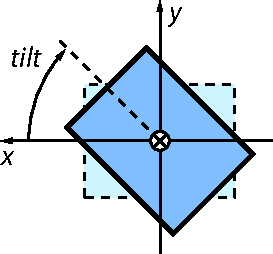
\includegraphics[width=\textwidth]{tilt.pdf}
    \caption{Effect of a tilt on a straight line element.}
    \label{f:tilt}
  \end{subfigure}
  \caption{}
\end{figure}

Once the \vn{reference} coordinate system is established, The position of any physical element with straight geometry can
be shifted (``misaligned'') using the element attributes:
\begin{description}
\item[x_offset, y_offset, z_offset]
The \vn{x_offset}, \vn{y_offset}, and \vn{z_offset} attributes offset the element in the $x$, $y$,
and $z$ directions respectively. See Figure~\ref{f:pitch}.
\item[x_pitch, y_pitch]
The \vn{x_pitch} and \vn{y_pitch} attributes rotate the element. A \vn{x_pitch} of $\pi/2$ would rotate the
element around the +$y$-axis so that the body +$z$-axis is aligned with the local
+$x$-axis. Similarly, a \vn{y_pitch} of $\pi/2$ would rotate the element around the -$x$-axis so
that the body +$z$-axis is aligned with the local +$y$-axis. See Figure~\ref{f:pitch}.
\item[tilt]
A \vn{tilt} rotates the element around the +$z$-axis as shown in Figure~\ref{f:tilt}
\end{description}

Note: The above only applies to straight elements. Patch like elements are explained below. For a
discussion of misalignments for bend type elements see the \bmad manual.

Example:
\begin{code}
beginning[beta_a] = 10.   ! m  a-mode beta function
beginning[beta_b] = 10.   ! m  b-mode beta function
beginning[e_tot] = 10e6   ! eV
parameter[geometry] = open  ! or closed
q: quadrupole, L = 1, x_offset = 0.1, x_pitch = 0.04
lat: line = (q)   ! List of lattice elements
use, lat          ! Line used to construct the lattice
\end{code}

Copy this lattice to a file and run \tao with this lattice as explained in
section~\sref{s:tao.start}:

\begin{code} 
Tao> show ele q -floor

 Element #                1
 Element Name: Q

Global Floor Coords at End of Element:
                X        Y        Z    Theta  
Reference  0.00000  0.00000  1.00000  0.00000 ... ! Without misalignments
Actual     0.11999  0.00000  0.99960  0.04000 ... ! With misalignments
delta Ref  0.11999  0.00000  0.99960  0.04000 ... ! Delta from last element
\end{code}

The \vn{Reference} row shows the nominal position of the \vn{exit} end of the element without
misalignmnets. [Due to space constaraints the \vn{phi} and \vn{psi} columns are not shown. They are
zero in this case.] The \vn{Actual} row shows the position of the physical element at the \vn{exit} end.

\begin{figure}[tb]
  \centering
  \begin{subfigure}[b]{0.48\textwidth}
    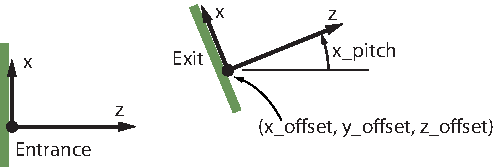
\includegraphics[width=\textwidth]{patch.pdf}
    \caption{The body coordinates at the exit end of a \vn{patch} is set by the element attributes
\vn{x_offset}, \vn{y_offset}, \vn{z_offset}, \vn{x_pitch}, \vn{y_pitch}, and \vn{tilt}.}
    \label{f:patch}
  \end{subfigure}
  \hfil
  \begin{subfigure}[b]{0.48\textwidth}
    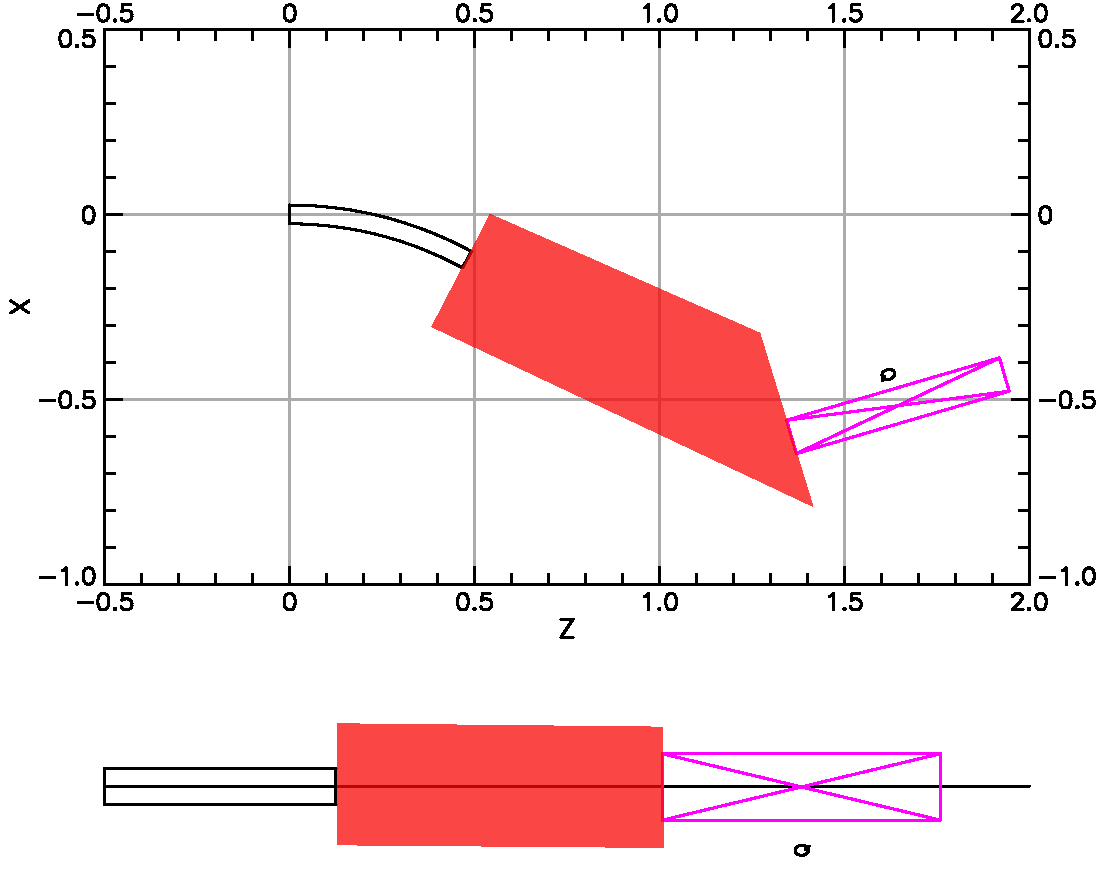
\includegraphics[width=\textwidth]{patch-example.pdf}
    \caption{Example use of a patch element in a lattice.}
    \label{f:patch.example}
  \end{subfigure}
  \caption{}
\end{figure}

%----------------------------------------------------------
\subsection{Patch Elements}

For \vn{patch} elements the same six parameters that are used to misalign straight line elements
are, for a \vn{patch}, use to set the placement of the \vn{exit} frame relative to the \vn{entrance}
frame.

The transformation from entrance coordinates to exit coordinate is:
\begin{enumerate}
\item Initially the exit coordinates coincide with the entrance coordinates.
\item The origin of the exit coordinates is translated by (\vn{x_offset}, \vn{y_offset}, \vn{z_offset})
\item The \vn{x_pitch} and \vn{y_pitch} rotations (in radians) are applied. 
The \vn{x_pitch} rotation rotates the \vn{+z} axis
towards the \vn{+x} axis (rotation around the +y axis). The \vn{y_pitch} rotation rotates the \vn{+z} axis
towards the \vn{+y} axis (rotation around the -x axis).
\item The \vn{tilt} rotation (in radians) rotates the exit coordinates around the exit coordinate's +z
axis.
\end{enumerate}
This transformation is illustrated in Figure~\ref{f:patch}. The transformation from \vn{patch}
\vn{entrance} to \vn{exit} coordinates is the same transformation from laboritory coordinates at the
center of a straight element to the element body coordinates at the center of the misaligned
element.

Example:
\begin{code}
beginning[beta_a] = 10.   ! m  a-mode beta function
beginning[beta_b] = 10.   ! m  b-mode beta function
beginning[e_tot] = 10e6   ! eV
parameter[geometry] = open  ! or closed

b: sbend, L = 0.5, g = 1    ! g = 1 / bending_radius
p: patch, z_offset = 1, x_pitch = pi/4
q: quadrupole, L = 0.6, k1 = 0.23

lat: line = (b, p, q)   ! List of lattice elements
use, lat                ! Line used to construct the lattice
\end{code}

Copy this lattice to a file and run \tao with this lattice as explained in
section~\sref{s:tao.start} and create a \vn{floor_plan} with the command 
\vn{place r11 floor}. The result is shown in Figure~\ref{f:patch.example}.
By default, \vn{patch} elements are not drawn but the global coordinates
of the elements can be seen by using the \vn{show lat -fllor} command:
\begin{code}
Tao> show lat -floor

      Values at End of Element:
 Index  name      key               s           X           Y           Z       Theta ...
     0  BEGINNING Beginning_Ele  0.000     0.00000     0.00000     0.00000     0.00000 ...
     1  B         Sbend          0.500    -0.12242     0.00000     0.47943    -0.50000 ...
     2  P         Patch          1.207    -0.60184     0.00000     1.35701     0.28540 ...
     3  Q         Quadrupole     1.807    -0.43292     0.00000     1.93274     0.28540 ...
     4  END       Marker         1.807    -0.43292     0.00000     1.93274     0.28540 ...
 Index  name      key                s           X           Y           Z       Theta ...
      Values at End of Element:
\end{code}

%----------------------------------------------------------
\Section{Particle Phase Space Coordinates}

The previous section showed how to describe the placement of lattice elements. This section
covers how to describe particle trajectories. 


\begin{figure}[tb]
  \centering
  \begin{subfigure}[b]{0.48\textwidth}
    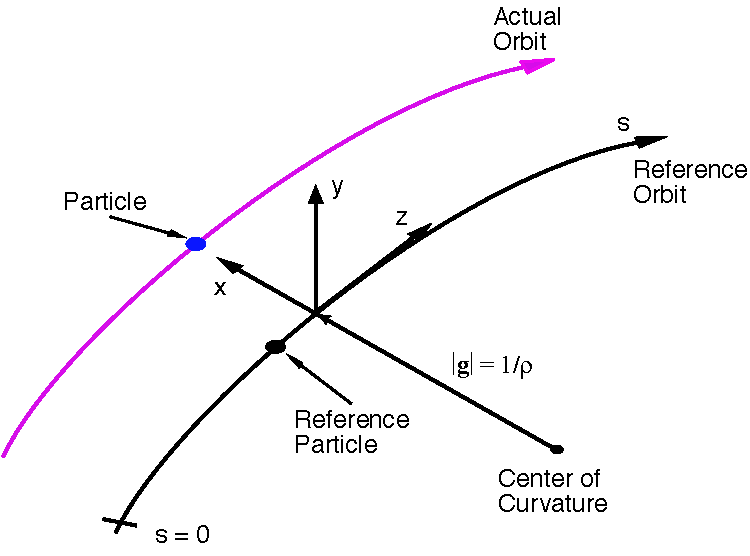
\includegraphics[width=0.9\textwidth]{local-coords.pdf}
    \caption{Particle coordinate positions are relative to the reference orbit.}
    \label{f:part.coords}
  \end{subfigure}
  \hfil
  \begin{subfigure}[b]{0.48\textwidth}
    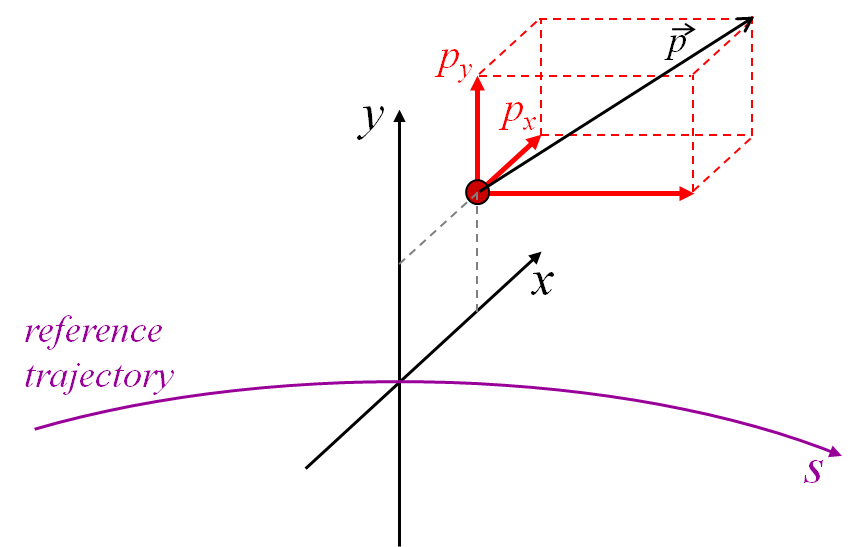
\includegraphics[width=\textwidth]{CoordinateSystem1.pdf}
    \caption{Particle phase space.}
    \label{f:phase.space}
  \end{subfigure}
  \caption{}
\end{figure}

%----------------------------------------------------------
\subsection{Particle Phase Space Coordinates}

Given a particle at some point on its trajectory, there is a reference frame on the reference orbit
at some \vn{s} value such that the particle's position is in the x-y plane with z = 0 as shown
in Figure~\ref{f:part.coords}. The
particle's particle's position and momentum \vn{P} can be described using the coordinates:
\begin{code}
    (x(s), y(s), Px(s), Py(s), Pz(s), t(s))
\end{code}

For tracking purposes, canonical phase space coordinates are used:
\begin{code}
    (x, px, y, py, z, pz)   
\end{code}
[Note convention: Upper case \vn{P} = (unnormalized) momentum. Lower case \vn{p} = phase space momentum]

where
\begin{code}
    px = Px / P0
    py = Py / P0
    pz = (P - P0) / P0
    z  = c * $\beta$ * (t_ref - t)
\end{code}

where 
\begin{itemize}
\item \vn{P0} is the reference momentum, 
\item \vn{$\beta$} is the velocity of the particle, 
\item \vn{t_ref(s)} is the time the reference particle reaches the point \vn{s}.
\end{itemize}

This is illustrated in Figure~\ref{f:phase.space}.

Notes:
\begin{itemize}
\item For a bunch of particles at a given \vn{s} position, in general the particles will have differing \vn{t}.
\item If the reference particle has the same $\beta$ value as a particle, canonical \vn{z} will be the longitudinal distance 
the particle is with respect to the reference particle. Positive \vn{z} indicates that the particle
is in front of the reference particle.
\end{itemize}


\begin{figure}[tb]
  \centering
  \begin{subfigure}[b]{0.48\textwidth}
    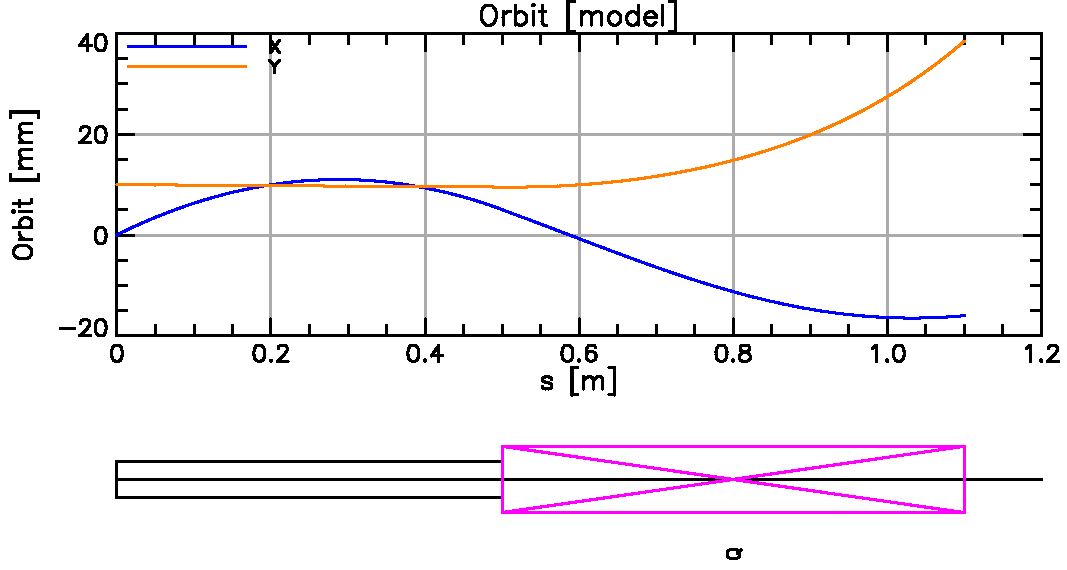
\includegraphics[width=\textwidth]{phase0.pdf}
    \caption{Initial orbit.}
    \label{f:phase0}
  \end{subfigure}
  \hfil
  \begin{subfigure}[b]{0.48\textwidth}
    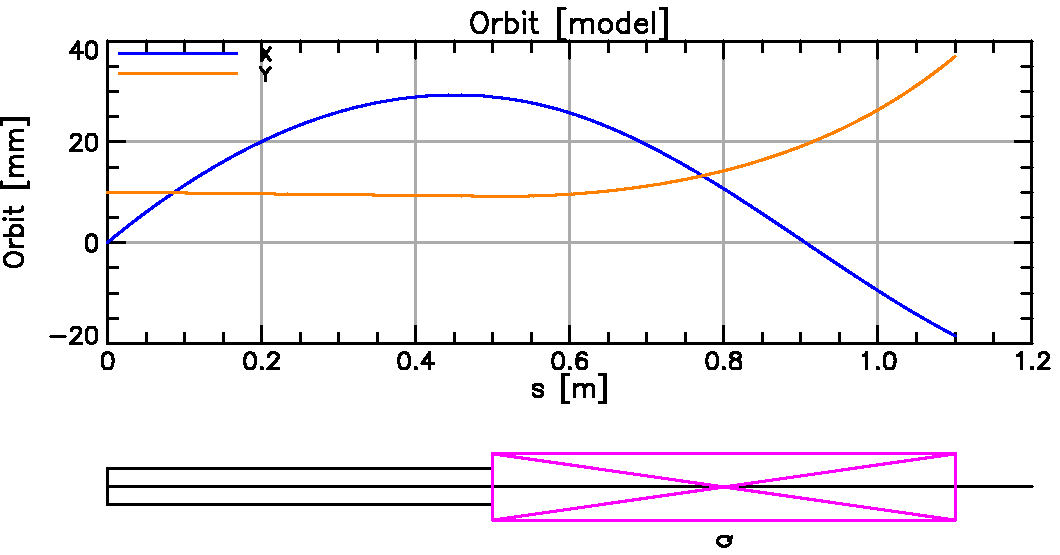
\includegraphics[width=\textwidth]{phase1.pdf}
    \caption{Orbit after adjusting the starting \vn{px} phase space coordinate.}
    \label{f:phase1}
  \end{subfigure}
  \caption{}
\end{figure}

%----------------------------------------------------------
\subsection{Example}

Example lattice:
\begin{code}
beginning[beta_a] = 10.     ! m  a-mode beta function
beginning[beta_b] = 10.     ! m  b-mode beta function
beginning[e_tot] = 10e6     ! eV
parameter[geometry] = open  ! or closed

beam_start[y] = 0.01
beam_start[px] = 0.06
beam_start[pz] = -0.2

b: sbend, L = 0.5, g = 1    ! g = 1 / bending_radius
q: quadrupole, L = 0.6, k1 = 10

lat: line = (b, q)      ! List of lattice elements
use, lat                ! Line used to construct the lattice
\end{code}

Copy this lattice to a file and run \tao with this lattice as explained in
section~\sref{s:tao.start}. The resulting orbit is shown in Figure~\ref{f:phase0}.


Now the initial phase space coordinates can be varied using the \vn{change} or \vn{set}
commands. For example:
\begin{code}
> tao -lat phase_space.bmad

Tao> change beam_start px 0.04
           Old           New    Old-Design    New-Design         Delta
      0.060000      0.100000      0.000000      0.040000      0.040000    BEAM_START
\end{code}

The result is shown in Figure~\ref{s:phase1}.

View Orbits with \vn{show lattice} caommand

\begin{code}
Tao> show lat
      Values at End of Element:
 Index  name      key                       s       l    beta     phi    eta  orbit     beta     phi    eta  orbit    Track_State
                                                            a       a      a  x [mm]       b       b      b  y [mm]
     0  BEGINNING Beginning_Ele         0.000     ---   10.00   0.000   0.00   0.000   10.00   0.000   0.00  10.000   Alive
     1  B         Sbend                 0.500   0.500    7.62   0.069   0.20  28.889    8.51   0.069   0.01   9.201   Alive
     2  Q         Quadrupole            1.100   0.600    3.60   3.153   0.11 -18.477  138.05   0.112  -0.00  36.926   Alive
     3  END       Marker                1.100   0.000    3.60   3.153   0.11 -18.477  138.05   0.112  -0.00  36.926   Alive
 Index  name      key                       s       l    beta     phi    eta  orbit     beta     phi    eta  orbit    Track_State
                                                            a       a      a  x [mm]       b       b      b  y [mm]
      Values at End of Element:
\end{code}

or the \vn{show element} command

\begin{code}
Tao> show ele 0
 Element #                0
 Element Name: BEGINNING
 Key: Beginning_Ele

... etc...

Orbit:  Positron   State: Alive
         Position[mm] Momentum[mrad]        Spin   |
  X:       0.00000000   100.00000000               | Particle [sec]:      0.00000000E+00  E_tot;  8.0059E+06
  Y:      10.00000000     0.00000000               | Part-Ref [sec]:      0.00000000E+00  PC:     7.9895E+06
  Z:       0.00000000  -200.00000000               | (Ref-Part)*Vel [m]:  0.00000000E+00  Beta:    0.997961
\end{code}

%----------------------------------------------------------
\subsection{Reference Energy and the Lcavity and RFcavity Elements}


\vn{Lcavity} and \vn{RFcavity}  elements are RF cavity elements. The difference is that the reference
 energy at the exit end of an \vn{lcavity} is shifted from the reference energy at the beginning
 while \vn{rfcavity} elements do not affect the reference energy. Example:
\begin{code}
beginning[beta_a] = 10.   ! m  a-mode beta function
beginning[beta_b] = 10.   ! m  b-mode beta function
beginning[p0c] = 1e8   ! eV  

parameter[geometry] = open      ! or closed
parameter[particle] = He+ 

q1: quad, l = 0.1, k1 = 0.14
q2: quad, l = 0.1, b1_gradient = parameter[p0c] * q1[k1] / c_light
lc: lcavity, l = 1, voltage = 10e8, rf_frequency = 1e9
rf: rfcavity, l = 1, voltage = 10e8, phi0 = 0.25

lat: line = (q1, q2, lc, q1, q2, rf)
use, lat
\end{code}

Notes:
\begin{itemize}
\item For a \vn{lcavity} phi0 = 0 corresponds to peak acceleration.
\item For an \vn{rfcavity} phi0 = 0.25 corresponds to peak acceleration.
\end{itemize}

Copy this lattice to a file and run \tao with this lattice as explained in
section~\sref{s:tao.start}.

\begin{code}
> tao -lat cavity.bmad

Tao> show ele 3
Element #                3
Element Name: LC
Key: Lcavity
... etc...
   51   P0C_START                    =  1.0000000E+08 eV            BETA_START      =  0.026811514
   52   E_TOT_START                  =  3.7297409E+09 eV            DELTA_E         =  1.0000000E+09 eV
   53   P0C                          =  2.9102374E+09 eV            BETA            =  0.615305883
   54   E_TOT                        =  4.7297409E+09 eV            GAMMA           =  1.2685712E+00
... etc...    
Orbit:  He+   State: Alive
         Position[mm] Momentum[mrad]        Spin   |
  X:       0.00000000     0.00000000               | Particle [sec]:      3.42560963E-08  E_tot;  4.7297E+09
  Y:       0.00000000     0.00000000               | Part-Ref [sec]:      0.00000000E+00  PC:     2.9102E+09
  Z:      -0.00000000     0.00000000               | (Ref-Part)*Vel [m]:  0.00000000E+00  Beta:    0.615306

Tao> show ele 6
Element #                6
Element Name: RF
Key: RFcavity
... etc...
   53   P0C                          =  2.9102374E+09 eV            BETA            =  0.615305883
   54   E_TOT                        =  4.7297409E+09 eV            GAMMA           =  1.2685712E+00
... etc...
 Orbit:  He+   State: Alive
         Position[mm] Momentum[mrad]        Spin   |
  X:       0.00000000     0.00000000               | Particle [sec]:      4.01447790E-08  E_tot;  5.7297E+09
  Y:       0.00000000     0.00000000               | Part-Ref [sec]:     -6.16649425E-10  PC:     4.3507E+09
  Z:     140.37425587   494.97867675               | (Ref-Part)*Vel [m]:  1.40374256E-01  Beta:    0.759326
\end{code}

Questions:
\begin{itemize}
\item What are the k1 and b1_gradient values for the first q1 and the second q1? Do you understand this?
\item What are the k1 and b1_gradient values for the first q2 and the second q2?
\end{itemize}

%----------------------------------------------------------
\Section{Superposition}

Superposition is used when elements overlap spatially. In such a case Bmad creates \vn{slave} elements that will be tracked through
and \vn{lord} elements that represent the individual elements.


\begin{figure}[tb]
  \centering
  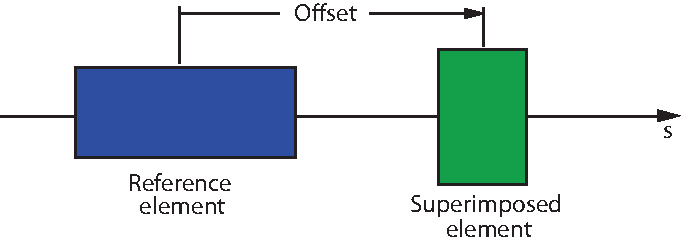
\includegraphics[width=0.9\textwidth]{superimpose.pdf}
  \caption{The placement of superimposed elements is determined by an offset from a reference element.}
  \label{f:superimpose}
\end{figure}

%----------------------------------------------------------
\subsection{Example 1}

To superimpose an element you need to specify where the element is placed. To do this, a reference position is specified
and the superimposed element is placed at that position shifted by a specified offset.

\begin{code}
beginning[beta_a] = 10.   ! m  a-mode beta function
beginning[beta_b] = 10.   ! m  b-mode beta function
beginning[e_tot] = 10e6   ! eV   Or can set p0c
parameter[geometry] = open      ! or closed

q: quadrupole, L = 1, k1 = 0.2
d: drift, L = 1

m1: marker, superimpose, ref = q, ref_origin = beginning, offset = 0.3
m2: marker, superimpose, ref = q, ref_origin = end, offset = 0.4

lat: line = (q, d)   ! List of lattice elements
use, lat             ! Line used to construct the lattice
\end{code}

Copy this lattice to a file and run \tao with this lattice as explained in
section~\sref{s:tao.start}. 

\begin{code}
> tao -lat superimpose.bmad

Tao> show lat
      Values at End of Element:
 Index  name      key                       s       l    beta     phi    eta  orbit     beta     phi    eta  orbit    Track_State
                                                            a       a      a  x [mm]       b       b      b  y [mm]
     0  BEGINNING Beginning_Ele         0.000     ---   10.00   0.000   0.00   0.000   10.00   0.000   0.00   0.000   Alive
     1  Q#1       Quadrupole            0.300   0.300    9.83   0.030   0.00   0.000   10.19   0.030   0.00   0.000   Alive
     2  M1        Marker                0.300   0.000    9.83   0.030   0.00   0.000   10.19   0.030   0.00   0.000   Alive
     3  Q#2       Quadrupole            1.000   0.700    8.22   0.107   0.00   0.000   12.24   0.094   0.00   0.000   Alive
     4  D#1       Drift                 1.400   0.400    6.97   0.160   0.00   0.000   14.24   0.124   0.00   0.000   Alive
     5  M2        Marker                1.400   0.000    6.97   0.160   0.00   0.000   14.24   0.124   0.00   0.000   Alive
     6  D#2       Drift                 2.000   0.600    5.37   0.258   0.00   0.000   17.58   0.162   0.00   0.000   Alive
     7  END       Marker                2.000   0.000    5.37   0.258   0.00   0.000   17.58   0.162   0.00   0.000   Alive
 ord Elements:
     8  Q         Quadrupole            1.000   1.000    8.22   0.107   0.00   0.000   12.24   0.094   0.00   0.000   Alive
 Index  name      key                       s       l    beta     phi    eta  orbit     beta     phi    eta  orbit    Track_State
                                                            a       a      a  x [mm]       b       b      b  y [mm]
      Values at End of Element:
\end{code}

The quadrupole \vn{Q} has been split by marker \vn{M1}. The two \vn{super_slave} elements \vn{Q\#1}
and \vn{Q\#2} will be used when tracking a particle through the lattice.

\begin{code}
Tao> show ele Q#1
 Element #                1
 Element Name: Q#1
 Key: Quadrupole
... etc...

Slave_status: Super_Slave
Associated Super_Lord(s):
   Index   Name                             Type
       8   Q                                Quadrupole
Lord_status:  Not_a_Lord
\end{code}

The \vn{Q} \vn{super_lord} element represents the actual quadrupole.
\begin{code}
Tao> show ele Q
 Element #                8
 Element Name: Q
 Key: Quadrupole
... etc...

Slave_status: Free
Lord_status:  Super_Lord
Slaves:
   Index   Name        Type
       1   Q#1         Quadrupole
       3   Q#2         Quadrupole
\end{code}

If parameters of element \vn{Q} are modified, Bmad bookkeeping routines will automatically update the super_slaves.
\begin{code}
Tao> change ele Q k1 0.11
           Old           New    Old-Design    New-Design         Delta
      0.200000      0.310000      0.110000      0.110000      0.110000    Q

Tao> show ele 1
 Element #                1
 Element Name: Q#1
 Key: Quadrupole
 S_start, S:    0.000000,    0.300000
 Ref_time:  1.002001E-09

 Attribute values [Only non-zero/non-default values shown]:
    1   L                            =  3.0000000E-01 m
    4   K1                           =  3.1000000E-01 1/m^2
... etc...
\end{code}

Parameter values of the super_slave elements may not be directly set:
\begin{code}
Tao> change ele Q#1 k1 0.01
[ERROR | 2017-AUG-28 22:38:36] tao_change_ele:
    ATTRIBUTE NOT FREE TO VARY. NOTHING DONE
\end{code}

Notes:
\begin{itemize}
\item No super_lord element is made when a drift element is split. Thus in the above example, there is no \vn{D} super_lord and
the two elements \vn{D\#1} and \vn{D\#1} and \vn{not} super_slaves.
\end{itemize}

%----------------------------------------------------------
\subsection{Example 2}


A more complicated example involving superposition of an element with finite length:
\begin{code}
beginning[beta_a] = 10.   ! m  a-mode beta function
beginning[beta_b] = 10.   ! m  b-mode beta function
beginning[e_tot] = 10e6   ! eV   Or can set p0c
parameter[geometry] = open      ! or closed

Q: quad, l = 4
D: drift, l = 12
S: solenoid, l = 8, superimpose, ref = Q, ele_origin = beginning
M: marker, superimpose, ref = S, offset = 1

lat: line = (Q, D)
use, lat
\end{code}

Copy this lattice to a file and run \tao with this lattice as explained in
section~\sref{s:tao.start}. 

\begin{code}
Tao> show lat
      Values at End of Element:
 Index  name      key                       s       l    beta     phi    eta  orbit     beta     phi    eta  orbit    Track_State
                                                            a       a      a  x [mm]       b       b      b  y [mm]
     0  BEGINNING Beginning_Ele         0.000     ---   10.00   0.000   0.00   0.000   10.00   0.000   0.00   0.000   Alive
     1  Q#1       Quadrupole            2.000   2.000   10.40   0.197   0.00   0.000   10.40   0.197   0.00   0.000   Alive
     2  Q\S       Sol_Quad              4.000   2.000   11.60   0.381   0.00   0.000   11.60   0.381   0.00   0.000   Alive
     3  S#1       Solenoid              7.000   3.000   14.90   0.611   0.00   0.000   14.90   0.611   0.00   0.000   Alive
     4  M         Marker                7.000   0.000   14.90   0.611   0.00   0.000   14.90   0.611   0.00   0.000   Alive
     5  S#2       Solenoid             10.000   3.000   20.00   0.785   0.00   0.000   20.00   0.785   0.00   0.000   Alive
     6  D#1       Drift                16.000   6.000   35.60   1.012   0.00   0.000   35.60   1.012   0.00   0.000   Alive
     7  END       Marker               16.000   0.000   35.60   1.012   0.00   0.000   35.60   1.012   0.00   0.000   Alive
Lord Elements:
     8  Q         Quadrupole            4.000   4.000   11.60   0.381   0.00   0.000   11.60   0.381   0.00   0.000   Alive
     9  S         Solenoid             10.000   8.000   20.00   0.785   0.00   0.000   20.00   0.785   0.00   0.000   Alive
 Index  name      key                       s       l    beta     phi    eta  orbit     beta     phi    eta  orbit    Track_State
                                                            a       a      a  x [mm]       b       b      b  y [mm]
      Values at End of Element:
\end{code}

The \vn{Q\S} super_slave element has both \vn{Q} and \vn{S} elements as super_lords
\begin{code}
Tao> show ele q\s
 Element #                2
 Element Name: Q\S
... etc...

Slave_status: Super_Slave
Associated Super_Lord(s):
   Index   Name                             Type
       8   Q                                Quadrupole
       9   S                                Solenoid
Lord_status:  Not_a_Lord
\end{code}

Notes:
\begin{itemize}
\item This superposition works since Bmad has a \vn{sol_quad} element which is a combination solenoid/quadrupole. It is not possible
to superimpose a quadrupole with a sextupole since Bmad does not have a combination quadrupole/sextupole element.
\item With closed lattices, a superimposed element may "wrap" around so that part of the superimposed element is at the end of the lattice
and part of the element is at the beginning of the lattice.
\end{itemize}

%----------------------------------------------------------
\Section{Multipass}

Some lattices have the beam recirculating through the same element multiple times. For example, an
Energy Recovery Linac (ERL) will circulate the beam back through the LINAC part to retrieve the
energy in the beam. In \bmad, this situation can simulated by designating the LINAC section as \vn{multipass}. 

%----------------------------------------------------------
\subsection{What is Multipass and What is it Good For?}

Consider the following lattice:
\begin{code}
A: quadrupole
ll: line = (A, A)
use, ll
\end{code}
The lattice has two elements both called \vn{A}. These two elements, even though they have the same name, are independent.
\begin{code}
Tao> change ele 1 k1 0.01   ! Can modify first A element.
Tao> change ele 2 k1 0.02   ! And can modify second A element independently.
\end{code}
With an ERL the beam will go through the linac section multiple times
\begin{code}
linac: line = (...)
arc: line = (...)
erl_line: line = (injector, linac, arc, linac, ...)
\end{code}
Here you don't want the elements of the fist \vn{linac} in \vn{erl_line} to be treated as separate
from the second \vn{linac} in \vn{erl_line} since they represent the same set of physical elements.
This is where \vn{multipass} comes in.  Multipass is used to describe the situation where a beam
recirculates through the same physical set of elements multiple times.

Essentially the solution is to mark the \vn{linac} line as multipass to tell Bmad that the first instance of \vn{linac} in \vn{erl_line}
contains the same physical elements as the second instance of \vn{linac}:
\begin{code}
linac: line[multipass] = (...)
\end{code}

%----------------------------------------------------------
\subsection{Example}

\begin{code}
beginning[beta_a] = 100.   ! m  a-mode beta function
beginning[beta_b] = 100.   ! m  b-mode beta function
beginning[p0c] = 10e6   ! eV   

parameter[geometry] = open      ! or closed

cavity: lcavity, l = 1, voltage = 10e6

linac: line[multipass] = (cavity)
erl: line = (linac, linac) 
use, erl

expand_lattice                
cavity\2[phi0_multipass] = 0.5
\end{code}

Copy this lattice to a file and run \tao with this lattice as explained in
section~\sref{s:tao.start}. 


\begin{code}
Tao> show lat

Tao> show lat
      Values at End of Element:
 Index  name      key                       s       l    beta     phi    eta  orbit     beta     phi    eta  orbit    Track_State
                                                            a       a      a  x [mm]       b       b      b  y [mm]
     0  BEGINNING Beginning_Ele         0.000     ---  100.00   0.000   0.00   0.000  100.00   0.000   0.00   0.000   Alive
     1  CAVITY\\1  Lcavity               1.000   1.000   78.87   0.011  -0.00   0.372   78.87   0.011   0.00   0.000   Alive
     2  CAVITY\\2  Lcavity               2.000   1.000   42.09   0.028  -0.00   0.352   42.09   0.028   0.00   0.000   Alive
     3  END       Marker                2.000   0.000   42.09   0.028  -0.00   0.352   42.09   0.028   0.00   0.000   Alive
Lord Elements:
     4  CAVITY    Lcavity               0.000   1.000    0.00   0.000   0.00     ---    0.00   0.000   0.00     ---   Not_Set
 Index  name      key                       s       l    beta     phi    eta  orbit     beta     phi    eta  orbit    Track_State
                                                        a       a      a  x [mm]       b       b      b  y [mm]
  Values at End of Element:
\end{code}

Bmad creates a \vn{multipass_lord} called \vn{cavity} to control the \vn{multipass_slaves} called
\vn{cavity\\1} and \vn{cavity\\2}:
\begin{code}
Tao> show ele 4
 Element #                4
 Element Name: CAVITY
... etc...
Slave_status: Free
Lord_status:  Multipass_Lord
Slaves:
   Index   Name        Type
       1   CAVITY\\1    Lcavity
       2   CAVITY\\2    Lcavity
\end{code}

Since the \vn{cavity} element represents the physical element, any change in the parameters of \vn{cavity}
will be be reflected in the slaves:
\begin{code}
Tao> set ele cavity x_offset = 0.001

Tao> show ele 2
 Element #                2
 Element Name: CAVITY\\2
 Key: Lcavity
 S_start, S:    1.000000,    2.000000
 Ref_time:  6.675633E-09

 Attribute values [Only non-zero/non-default values shown]:
    1   L                            =  1.0000000E+00 m
... etc...
   36   X_OFFSET                     =  1.0000000E-03 m        57   X_OFFSET_TOT    =  1.0000000E-03 m
... etc...
\end{code}

The exception to the rule that the multipass_lord completely controls the multipass_slave attributes
is the \vn{phi0_multipass} attribute of \vn{lcavity} and \vn{rfcavity} elements. \vn{phi0_multipass}
allows for different settings of the RF phase for different passes through the cavity element.
From the above lattice:
\begin{code}
expand_lattice                 ! cavity\2 is created during lattice expansion
cavity\2[phi0_multipass] = 0.5 ! This shifts the RF phase for cavity\2 by 180^deg
\end{code}
Giving:
\begin{code}
Tao> show lat -attrib e_tot
      Values at End of Element:
 Index  name      key                      s       l           e
                                                             tot
     0  BEGINNING Beginning_Ele        0.000     ---  1.0013E+07
     1  CAVITY\1  Lcavity              1.000   1.000  2.0013E+07
     2  CAVITY\2  Lcavity              2.000   1.000  1.0013E+07
     3  END       Marker               2.000   0.000  1.0013E+07
Lord Elements:
     4  CAVITY    Lcavity              0.000   1.000  2.0013E+07
 Index  name      key                      s       l           e
                                                             tot
\end{code}

Notes:
\begin{itemize}
\item Bmad does not demand that the global position of the multipass_slaves of a multipass_lord be in
the same position in the global coordinate system.
\end{itemize}

\begin{figure}[tb]
  \centering
  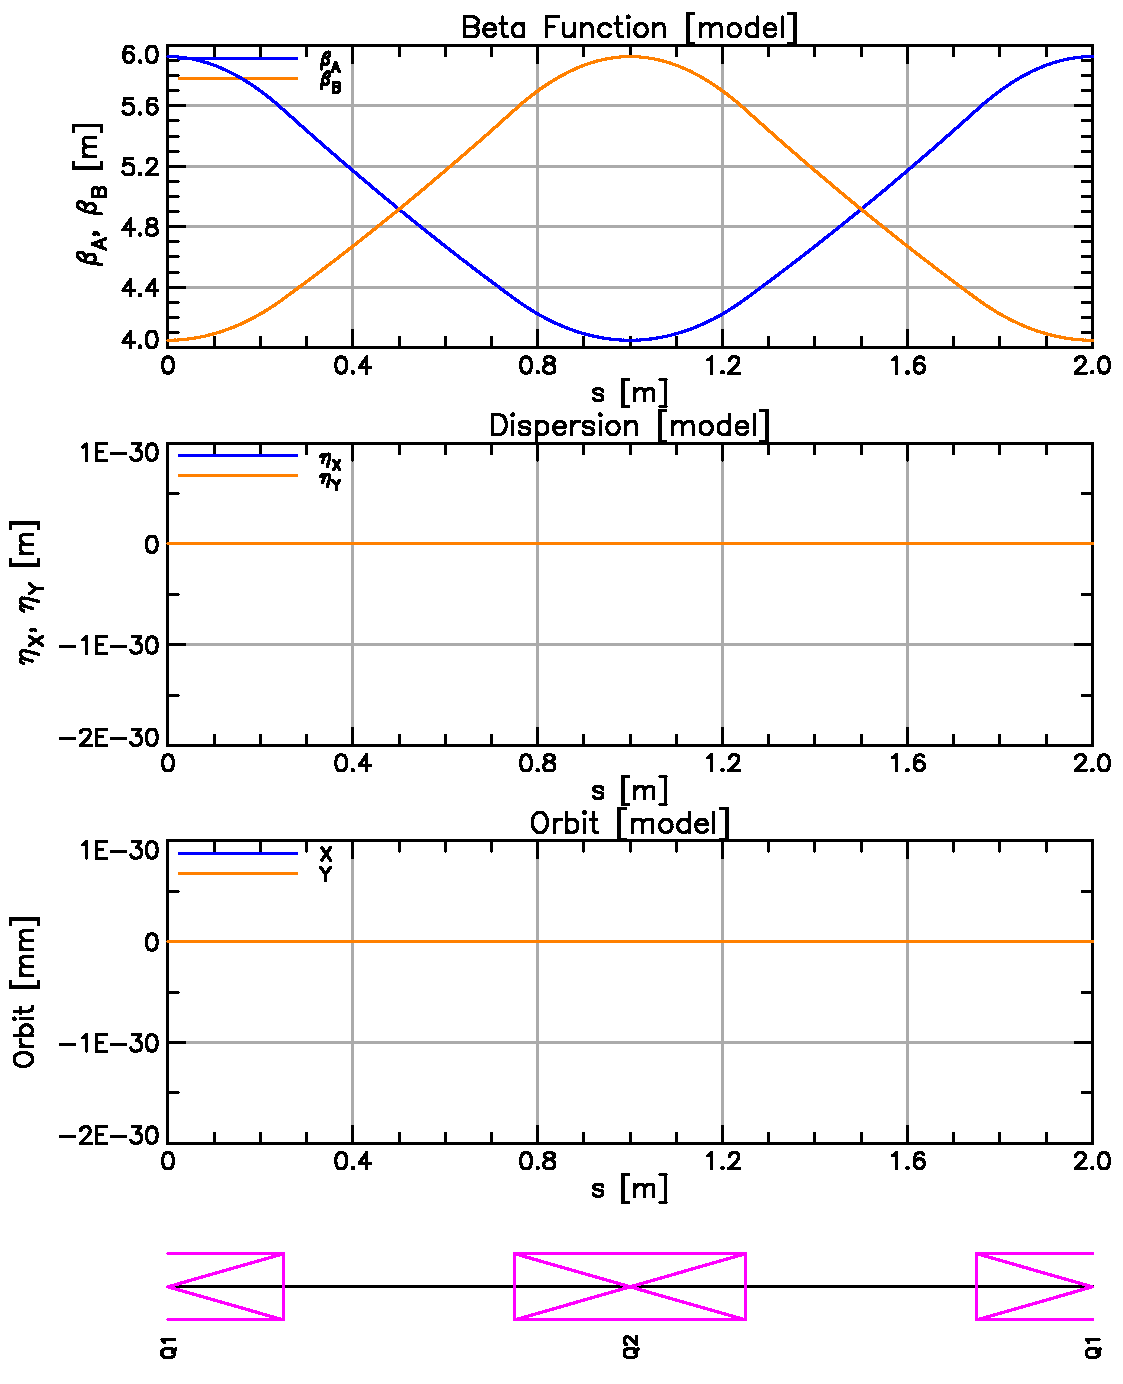
\includegraphics[width=0.9\textwidth]{geometry.pdf}
  \caption{\bmad computes the periodic Twiss and orbits for \vn{closed} lattices.}
  \label{f:geometry}
\end{figure}

%----------------------------------------------------------
\Section{Lattice Geometry}

The \vn{parameter[geometry]} parameter in a lattice file sets the lattice topology to:
\begin{description}
\item \vn{open}: For Twiss and reference orbit calculations Bmad uses the initial Twiss 
and orbit settings in the lattice for the beginning of the lattice and
propagates them to the end of the lattice (like you would do for a linac). 
\item \vn{closed}: For Twiss and reference orbit calculations, Bmad calculates the 
periodic solution (like you would in a storage ring). 
Bmad will ignore Twiss and orbit settings.
\end{description}

Example:
\begin{code}
parameter[p0c] = 1e9
parameter[geometry] = closed

d: drift, l = 2
q1: quad, l = 0.5, k1 = 3, hkick = 0.001, superimpose
q2: quad, l = 0.5, k1 = -3, vkick = 0.002, superimpose, offset = 1

lat: line = (d)
use, lat
\end{code}

The result is shown in Figure~\ref{f:geometry}:



\begin{code}
Tao> show lat
      Values at End of Element:
 Index  name      key                       s       l    beta     phi    eta  orbit     beta     phi    eta  orbit    Track_State
                                                            a       a      a  x [mm]       b       b      b  y [mm]
     0  BEGINNING Beginning_Ele         0.000     ---    5.93   0.000   0.00   0.000    4.05   0.000   0.00   0.000   Alive
     1  Q1#2      Quadrupole            0.250   0.250    5.57   0.043   0.00   0.000    4.32   0.060   0.00   0.000   Alive
     2  D#1       Drift                 0.750   0.500    4.32   0.145   0.00   0.000    5.57   0.162   0.00   0.000   Alive
     3  Q2        Quadrupole            1.250   0.500    4.32   0.266   0.00   0.000    5.57   0.249   0.00   0.000   Alive
     4  D#2       Drift                 1.750   0.500    5.57   0.368   0.00   0.000    4.32   0.351   0.00   0.000   Alive
     5  Q1#1      Quadrupole            2.000   0.250    5.93   0.411   0.00   0.000    4.05   0.411   0.00   0.000   Alive
     6  END       Marker                2.000   0.000    5.93   0.411   0.00   0.000    4.05   0.411   0.00   0.000   Alive
Lord Elements:
     7  Q1        Quadrupole            0.250   0.500    5.57   0.043   0.00     ---    4.32   0.060   0.00     ---   Not_Set
 Index  name      key                       s       l    beta     phi    eta  orbit     beta     phi    eta  orbit    Track_State
                                                            a       a      a  x [mm]       b       b      b  y [mm]
      Values at End of Element:


Tao> show ele q1
 Element #                7
 Element Name: Q1
 Key: Quadrupole
 S_start, S:    1.750000,    0.250000
... etc...

Slave_status: Free
Lord_status:  Super_Lord
Slaves:
   Index   Name        Type
       5   Q1#1        Quadrupole
       1   Q1#2        Quadrupole
\end{code}

Notes:
\begin{itemize}
\item Bmad does not demand that a closed lattice be closed in the sense that the global position at the end of the lattice be the same as the beginning.
\end{itemize}


\begin{figure}[tb]
  \centering
  \begin{subfigure}[b]{0.48\textwidth}
    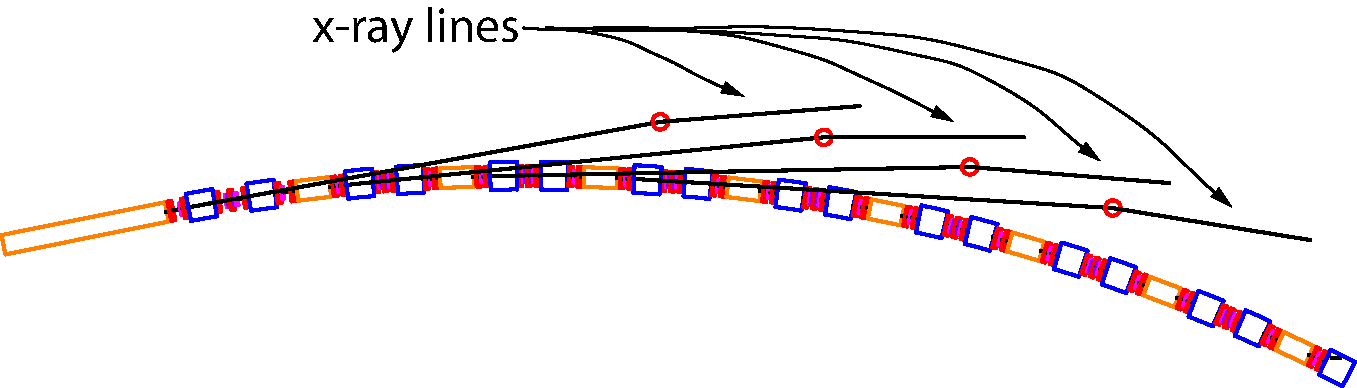
\includegraphics[width=\textwidth]{x-fork.pdf}
    \caption{Fork elements can be used to construct interconnected lines like x-ray lines branching
      from a storage ring.}
    \label{f:fork}
  \end{subfigure}
  \hfil
  \begin{subfigure}[b]{0.48\textwidth}
    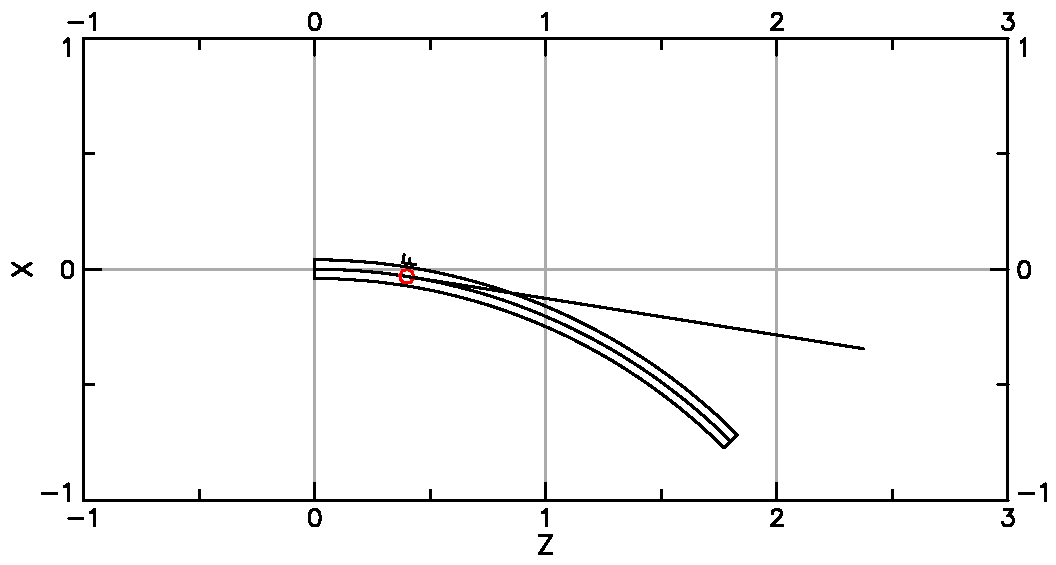
\includegraphics[width=\textwidth]{fork-example.pdf}
    \caption{Simple fork example.}
    \label{f:fork.example}
  \end{subfigure}
  \caption{}
\end{figure}

%----------------------------------------------------------
\Section{Forking Lines}

A \vn{fork} or \vn{photon_fork} element marks the point where multiple lines can merge or branch off from.
Forking elements can be used to describe X-ray lines branching from storage rings, injection or
extraction lines, etc. as shown in Figure~\ref{f:fork}

%----------------------------------------------------------
\subsection{Example}

\begin{code}
beginning[beta_a] = 10.0        ! m  a-mode beta function
beginning[beta_b] = 10.0        ! m  b-mode beta function
beginning[e_tot] = 10e6         ! eV 
parameter[geometry] = open      ! or closed

b: bend, l = 2, rho = pi/4
f: fork, to_line = extract_line, superimpose, offset = 0.4
d: drift, l = 2

extract_line: line = (d)       ! The line forked to.
extract_line[geometry] = open

lat: line = (b)
use, lat                ! Line used to construct the lattice
\end{code}

Copy this lattice to a file and run \tao with this lattice as explained in
section~\sref{s:tao.start}. 

\begin{code}
> tao -lat fork.bmad
Tao> place r11 floor
\end{code}

Gives Figure~\ref{f:fork.example}.
The lattice is looks like:

\begin{code}
Tao> show lat
      Values at End of Element:
 Index  name      key                       s       l    beta     phi    eta  orbit     beta     phi    eta  orbit    Track_State
                                                            a       a      a  x [mm]       b       b      b  y [mm]
     0  BEGINNING Beginning_Ele         0.000     ---   10.00   0.000   0.00   0.000   10.00   0.000   0.00   0.000   Alive
     1  B#1       Sbend                 0.400   0.400    9.77   0.040   0.03   0.000   10.02   0.040   0.00   0.000   Alive
     2  F         Fork                  0.400   0.000    9.77   0.040   0.03   0.000   10.02   0.040   0.00   0.000   Alive
     3  B#2       Sbend                 2.000   1.600    5.32   0.249   0.75   0.000   10.40   0.197   0.00   0.000   Alive
     4  END       Marker                2.000   0.000    5.32   0.249   0.75   0.000   10.40   0.197   0.00   0.000   Alive
Lord Elements:
     5  B         Sbend                 2.000   2.000    5.32   0.249   0.75   0.000   10.40   0.197   0.00   0.000   Alive
 Index  name      key                       s       l    beta     phi    eta  orbit     beta     phi    eta  orbit    Track_State
                                                            a       a      a  x [mm]       b       b      b  y [mm]
      Values at End of Element:
\end{code}

Where is the line that was forked to? Bmad creates \vn{branches} to hold the different
lines. Branches are assigned an index starting from 0:

\begin{code}
Tao> show branch
                          N_ele  N_ele                  Default                       Live
  Branch                  Track    Max   Ref_Particle   Tracking_Species    Geometry  Branch  From_Fork
  0: LAT                      4      5   Positron       Ref_Particle        Open       T
  1: EXTRACT_LINE             2      2   Positron       Ref_Particle        Open       T      0>>2
 
                                                                                                      Defines
  Fork_Element                              Forking_To                                   Direction    To_Branch?
  0>>2: LAT>>F                              1>>0: EXTRACT_LINE>>BEGINNING                 1             T
\end{code}  

The \vn{show lat} branch, by default, shows branch 0. To see other branches use the \vn{-branch} option:
\begin{code}
Tao> show lat -branch 1
      Values at End of Element:
 Index  name      key                       s       l    beta     phi    eta  orbit     beta     phi    eta  orbit    Track_State
                                                            a       a      a  x [mm]       b       b      b  y [mm]
     0  BEGINNING Beginning_Ele         0.000     ---    9.77   0.040   0.03   0.000   10.02   0.040   0.00   0.000   Alive
     1  D         Drift                 2.000   2.000    8.04   0.268   0.34   0.000   10.58   0.236   0.00   0.000   Alive
     2  END       Marker                2.000   0.000    8.04   0.268   0.34   0.000   10.58   0.236   0.00   0.000   Alive
 Index  name      key                       s       l    beta     phi    eta  orbit     beta     phi    eta  orbit    Track_State
                                                            a       a      a  x [mm]       b       b      b  y [mm]
      Values at End of Element:
\end{code}

Notes:
\begin{itemize}
\item The difference between \vn{fork} and \vn{photon_fork} is that the default species for \vn{fork} is
the same as the line forked from while for a \vn{photon_fork} the default species are photons.
\item A fork element is not restricted to forking to the beginning of a line. 
The place where a fork element connects can be set by the \vn{to_element} attribute.
\end{itemize}

%----------------------------------------------------------
\Section{Tracking Methods}

To each lattice element one can vary the method used to track particles through the element. This is
useful, among other things for optimizing speed and/or accuracy.
\begin{code}
    q1: quadrupole, l = 0.6, ..., tracking_method = runge_kutta
\end{code}

Some possibilities:
\begin{code}
\vn{bmad_standard}   Fast, thick element formulas.
\vn{symp_lie_ptc}    Symplectic Lee integration tracking.
\vn{taylor}          Taylor map.
\vn{linear}          Linear tracking.
\vn{custom}          Tracking with custom code.
\vn{runge_kutta}     Track through fields.
etc...
\end{code}

Much more information in the Bmad manual...


%----------------------------------------------------------
\Section{Data in Tao}

In order to optimize, you must tell Tao what quantities that you want to calculate that will contribute to the merit function. The basic structure has several: d2_data, which contains d1_data, which contains individual datums. You input these in the tao.init file as:
\begin{code}
&tao_d2_data
    d2_data%name = 'twiss'
    n_d1_data = 2
/
&tao_d1_data
    ix_d1_data = 1
    d1_data%name = 'end'
    datum( 1) =  'beta.a'     '' '' 'END'   'target'  12.5   1e1  
    datum( 2) =  'alpha.a'    '' '' 'END'   'target'  -1     1e2
/ 
&tao_d1_data
    ix_d1_data = 2
    d1_data%name = 'max'
    datum( 1) =  'beta.a'    '' 'Q1' 'END'   'max'  100   1e1
    datum( 2) =  'eta.x'     '' 'Q1' 'END'   'abs_max'  1     1e2
/ 
\end{code}

The first datum means that beta.a at element END should be 12.5 m with a weight of 10. If the model beta function is, say, 20 m at element END, then this datum would contribute $10*(20 - 12.5)^2$ to the merit function. 

The columns of an individual datum(i) are a shorthand input of the datum structure (type 'getf tao_datum_input' on the command line to see a full list). The columns are:
\begin{code}
data_type       ! Type of data: 'orbit.x', etc.
ele_ref_name    ! Name of reference lattice element
ele_start_name  ! Name of starting lattice element when there is a range
ele_name        ! Name of the lattice element where datum is evaluated.
merit_type      ! Type of constraint: 'target', 'max', 'min', etc.
meas            ! Measured datum value.
weight          ! Weight for the merit function term
\end{code}

In Tao, these can be shown with:
\begin{code}
Tao> show dat

  Name                                 Using for Optimization
  twiss.end[1:6]                                 Using: 1:6
  twiss.max[1:2]                                 Using: 1:2
\end{code}


%----------------------------------------------------------
\Section{Variables in Tao}



Variables must be defined in order to optimize. The simplest possible variable definition is: 
\begin{code}
    &tao_var
      v1_var%name = 'quad'
      default_step = 1e-4
      default_attribute = 'k1'
      search_for_lat_eles = 'Quad::*'
      ! or: 
      ! var(1:)%ele_name = 'Q1', 'Q2', 'Q3', 'Q4', 'Q5', 'Q6'
    /
\end{code}

This will search the lattice of all quadrupole key elements, and control their 'k1' attribute with a step of 1e-4.

In tao you will then see (if the elements exist) the variables in a short notation:
\begin{code}
Tao> sho var
       Name                                      Using for Optimization
    quad[1:6]
\end{code}

or a more detailed list:
\begin{code}
Tao> sho var quad
Variable name:  quad

 Index  Controlled Attributes(s)    Meas         Model        Design  Useit_opt
     1  Q1[K1]                  8.6924-311    0.0000E+00    0.0000E+00       F
     2  Q2[K1]                  8.6924-311    0.0000E+00    0.0000E+00       F
     3  Q3[K1]                  8.6924-311    0.0000E+00    0.0000E+00       F
     4  Q4[K1]                  8.6924-311    0.0000E+00    0.0000E+00       F
     5  Q5[K1]                  8.6924-311    0.0000E+00    0.0000E+00       F
     6  Q6[K1]                  8.6924-311    0.0000E+00    0.0000E+00       F
 Index  Controlled Attributes(s)    Meas         Model        Design  Useit_opt
\end{code}

A tao_var is an array of variables, each of which can have individually set attributes. Type: 
\begin{code}
Tao> sho var quad[2]
%ele_name         = Q2
%attrib_name      = K1
...
\end{code}

to see a complete list. Prepending: 'default_' in front of any of these in the variable definition will flag all variables to have the same property, like 'k1'. 

Variables can also have mixed properties, as in:
\begin{code}
var(1:4)%ele_name = 'FF.Qua01',  'FF.Qua02',  'FF.Qua02',  'O_quad_length'
var(1:4)%attribute = 'b1_gradient', 'b1_gradient', 'x_offset', 'f'
var(1:4)%key_delta = 0.1, 0.1, 0.0001, .01
var(1:4)%low_lim = -50, -50, -.1, .2
var(1:4)%high_lim = 50,  50,  .1, .8
\end{code}

Variable properties can also be changed within Tao. For example, 
\begin{code}
Tao> set var quad[1:4]|low_lim = -1
\end{code}
will set the lower limit for the first four quads.


%----------------------------------------------------------
\subsection{Key Bound Variables}


An alternative use for variables is to bind them to keys on the keyboard for use in Tao's 'Single Mode'. The two properties to set are %key_bound and %key_delta. In the input file, adding these properties as:
\begin{code}
&tao_var
  v1_var%name = 'quad'
  ...
  default_key_bound = T
  default_key_delta = 1e-2
/

Will then bind these variables to the keyboard keys 1-9, Q-O in single mode. For example,
\begin{code}
Tao> single
Entering Single Mode...
11>>111>>11qq>>>11
\end{code}

Enters single mode, and 1 raises the variable quad[1] by 1e-2, and q (the key under 1 on the keyboard) lowers it. The > and < signs change the default step by a factor of 2 or 1/2, which is useful when you would like the keys to make larger or smaller steps. The '11>>111>>11qq>>>11' is a history of what was pressed. 

To quit single mode, type upper case Z:
\begin{code}
Z
Entering line mode...
    
Tao> 
\end{code}


%----------------------------------------------------------
\Section{Using Tao for Optimization}






\end{document}



\begin{figure}[tb]
  \centering
  \begin{subfigure}[b]{0.48\textwidth}
    \includegraphics[width=\textwidth]{.pdf}
    \caption{}
    \label{f:}
  \end{subfigure}
  \hfil
  \begin{subfigure}[b]{0.48\textwidth}
    \includegraphics[width=\textwidth]{.pdf}
    \caption{.}
    \label{f:}
  \end{subfigure}
  \caption{}
\end{figure}

\begin{figure}[tb]
  \centering
  \includegraphics[width=0.9\textwidth]{.pdf}
  \caption{.}
  \label{f:}
\end{figure}
